% vim: set wrap


\documentclass{beamer} %[draft]
\usepackage{graphicx}
\usepackage{tikz}
\usetheme{default}
\useoutertheme{infolines}


\usepackage{tikz}
\usepackage{pgfplots}

\pgfplotsset{
  every axis legend/.append style={
    at={(1.01,1.0)},
    anchor=north west,
    font=\tiny, %\footnotesize,
  },
  width=10cm,
  height=6cm,
}

\usepackage{hyperref}

\usepackage{havannah}
\renewcommand\HDrawHex{\draw[fill=gray!35]}


\title{Playing and Solving Havannah}

\author[Timo Ewalds]{
	Timo Ewalds \\
	\texttt{timo@ewalds.ca}
}

\institute[UofA]{
	Department of Computing Science\\
	University of Alberta
}

%\setfootline{\insertshortauthor \hfill \insertshorttitle \hfill \insertshortdate \hfill \insertframenumber/\inserttotalframenumber}

\begin{document}


\begin{frame}[plain]
	\titlepage
\end{frame}

%\begin{frame}
%\begin{center}
%\Huge
%Playing and Solving Havannah
%\vspace{30pt}
%\huge
%Timo Ewalds
%\end{center}
%\end{frame}

%\begin{frame}{Overview}
%\begin{itemize}
%	\item Goal: Create a strong Havannah player, and solve boardsize 4
%	\item Background
%	\item Rules and Properties of Havannah
%	\item Playing Havannah
%	\item Solving Havannah
%	\item Conclusion
%\end{itemize}
%\end{frame}


\AtBeginSection[] % Do nothing for \section*
{
\begin{frame}{Outline}
\tableofcontents[currentsection, hideothersubsections]
\end{frame}
}


\begin{frame}{Outline}
\tableofcontents[hideallsubsections]
\end{frame}

%%%%%%%%%%%%%%%%%%%%%%%%%%%%%%%%%%%%%%%%%%%%%%%

\section{Introduction}

\begin{frame}{Motivation}
\begin{itemize}
	\item Artificial Intelligence (AI) is important
	\item Search is an important technique for AI
	\item Havannah is a good testcase for search
\end{itemize}
\end{frame}

\begin{frame}{Contributions}
\begin{itemize}
	\item Castro, open source
	\item Strong player
	\item Strong solver
	\item TODO ...
\end{itemize}
\end{frame}

%%%%%%%%%%%%%%%%%%%%%%%%%%%%%%%%%%%%%%%%%%%%%%%

\section{Background}

\subsection{Minimax, Alpha-Beta}

\begin{frame}{Minimax}
\begin{itemize}
	\item Basis of all game playing programs
	\item Minimize the maximum value your opponent can achieve.
\end{itemize}

\begin{figure}
\centering
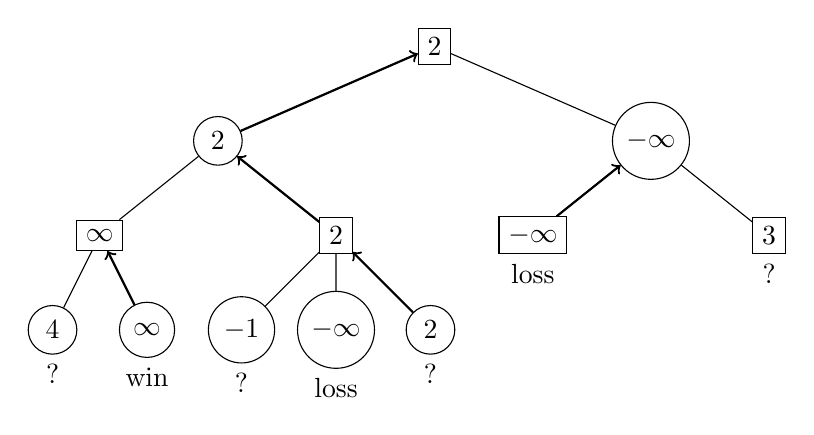
\begin{tikzpicture}[
	level distance=12mm,
	level 1/.style={sibling distance=55mm},
	level 2/.style={sibling distance=30mm},
	level 3/.style={sibling distance=12mm},
	]
\node [rectangle,draw] (a){$ 2 $}
  child {node (b) [circle,draw] {$ 2 $}
    child {node (d) [rectangle,draw] {$ \infty $}
      child {node (h) [circle,draw,label=below:?] {$ 4 $}}
      child {node (i) [circle,draw,label=below:win] {$ \infty $}}
    }
    child {node (e) [rectangle,draw] {$ 2 $}
      child {node (j) [circle,draw,label=below:?] {$ -1 $}}
      child {node (k) [circle,draw,label=below:loss] {$ -\infty $}}
      child {node (l) [circle,draw,label=below:?] {$ 2 $}}
    }
  }
  child {node (c) [circle,draw] {$ -\infty $}
    child {node (f) [rectangle,draw,label=below:loss] {$ -\infty $}}
    child {node (g) [rectangle,draw,label=below:?] {$ 3 $}}
  };
  \draw[thick,->] (b) -- (a);
  \draw[thick,->] (e) -- (b);
  \draw[thick,->] (i) -- (d);
  \draw[thick,->] (l) -- (e);
  \draw[thick,->] (f) -- (c);
\end{tikzpicture}
\caption[Minimax Tree]{Minimax Tree, squares are MAX nodes, circles are MIN nodes}
\label{fig:minimaxtree}
\end{figure}

\end{frame}

\begin{frame}{Alpha-Beta}
\begin{itemize}
	\item Maintains two values that bound the minimum value each player is guaranteed given the tree searched so far
	\item Given perfect move ordering, runs in $O(b^{d/2})$ instead of $O(b^d)$
	\item Refinements:
	\begin{itemize}
		\item Negamax Formulation
		\item Transposition Table
		\item Iterative Deepening
		\item History Heuristic
	\end{itemize}
	\item Used extensively in games with good heuristics, such as Chess
\end{itemize}
\end{frame}


\subsection{Proof Number Search}

\begin{frame}{Proof Number Search}
\begin{itemize}
	\item Best-first search to answer binary questions (solve a position)
	\item Represented with an AND/OR tree, analogous to MIN/MAX nodes
	\item Stores a Proof Number (PN) and Disproof Number (DN) for each position
	\item Most Proving Node (MPN) is a leaf node that, if solved, affects the root's PN or DN
	\item Continually expands a Most Proving Node
	\item Game/heuristic independent, guided towards parts of the tree where few options need to be solved
\end{itemize}
\end{frame}


\begin{frame}{Proof Number Search}
\begin{itemize}
	\item Finds MPN by selecting minimum PN at each OR node, minimum DN at each AND node.
	\item Expands children, set's PN = 1, DN = 1, or proven/disproven
	\item Backs up values with formulas: \\
	For OR nodes: $$ n.pn = \displaystyle\min\limits_{i=0}^k n_i.pn,\quad n.dn = \displaystyle\sum\limits_{i=0}^k n_i.dn $$ For AND nodes: $$ n.pn = \displaystyle\sum\limits_{i=0}^k n_i.pn, \quad n.dn = \displaystyle\min\limits_{i=0}^k n_i.dn $$
\end{itemize}
\end{frame}


%\begin{frame}{Proof Number Search}
%\begin{figure}
%\centering
%\begin{tikzpicture}[
%	level distance=15mm,
%	level 1/.style={sibling distance=60mm},
%	level 2/.style={sibling distance=35mm},
%	level 3/.style={sibling distance=15mm},
%	]
%\node [rectangle,draw] (z){$a \frac{1}{2}$}
%  child {node [circle,draw] {$b \frac{1}{2}$}
%    child {node [rectangle,draw] {$d \frac{0}{\infty}$}
%      child {node [circle,draw,label=below:?] {$h \frac{1}{1}$}}
%      child {node [circle,draw,label=below:win] {$i \frac{0}{\infty}$}}
%    }
%    child {node [rectangle,draw] {$e \frac{1}{2}$}
%      child {node [circle,draw,label=below:?] {$j \frac{1}{1}$}}
%      child {node [circle,draw,label=below:loss] {$k \frac{\infty}{0}$}}
%      child {node [circle,draw,label=below:?] {$l \frac{1}{1}$}}
%    }
%  }
%  child {node [circle,draw] {$c \frac{\infty}{0}$}
%    child {node [rectangle,draw,label=below:loss] {$f \frac{\infty}{0}$}}
%    child {node [rectangle,draw,label=below:?] {$g \frac{1}{1}$}}
%  };
%\end{tikzpicture}
%\caption[Proof Number Search Tree]{Proof Number Search Tree, squares are OR nodes, circles are AND nodes, proof numbers are on top, disproof numbers on the bottom
%\label{fig:pntree}
%\end{figure}
%\end{frame}


\subsection{Monte-Carlo Tree Search}

\begin{frame}{Monte-Carlo Tree Search}
\begin{itemize}
	\item Alpha-Beta only works for games with a good heuristic evaluation function
	\item Monte-Carlo evaluation can be used as a rough evaluation
	\item Tree search improves the evaluation by finding good replies
	\item Monte-Carlo Tree Search (MCTS) works well for several games
	\item MCTS consists of 4 phases: Descent, Expansion, Rollout and Back-propagation, together called a simulation
	\item MCTS runs simulations until time runs out or the position is solved
	\item Many extensions and variations to basic MCTS
\end{itemize}
\end{frame}


\begin{frame}{Monte-Carlo Tree Search}
\begin{figure}
	\centering
\includegraphics[width=0.9\textwidth]{mcts.pdf}
\caption[Four Phases of Monte Carlo Tree Search]{Four Phases of Monte Carlo Tree Search, together called a Simulation, shown in the negamax formulation with a minimum of 3 experience before expansion}
\label{fig:mcts}
\end{figure}
\end{frame}

\begin{frame}{Monte-Carlo Tree Search}
\begin{itemize}
	\item Many possible node selection policies for the descent phase
	\item Balance exploration and exploitation
	\item Use information from rollouts
	\item Heuristic knowledge
	\item Rollout Policy
\end{itemize}
\end{frame}


\begin{frame}{UCT}
\begin{itemize}
	\item Upper Confidence bounds as applied to Trees (UCT)
	\item Based on Upper Confidence Bounds (UCB) used for the multi-armed bandit problem
	\item $ n_i.v + c*\sqrt{\frac{\ln(n.n)}{n_i.n}} $
	\item Balances exploration vs exploitation in a theoretically optimal way
\end{itemize}
\end{frame}


\begin{frame}{RAVE}
\begin{itemize}
	\item A win in a rollout is composed of several good moves
	\item Moves that do well in rollouts are likely good if played earlier
	\item Winning rate for each move in rollouts can be tracked and combined with real experience: $$ \beta*n_i.v + (1-\beta)*n_i.r $$
	\item Phased out as real experience is gained, several possible formulas: $$ \beta = \frac{k}{k+n_i.n} \quad \beta = \frac{n_i.m}{n_i.n+n_i.m+4*n_i.n*n_i.m*b^2}$$
	\item RAVE often leads to sufficient exploration that UCT exploration term is removed
\end{itemize}
\end{frame}

\begin{frame}{Heuristic Knowledge}
\begin{itemize}
	\item UCT will find the right move eventually, but heuristics can help
	\item Uses game specific information to encourage exploration of likely good moves
	\item Can counteract unlucky randomness in rollouts
	\item Can be added as fake experience or as a separate term
	\item Fake experience initializes winning rate to non-zero values
	\item Separate term adds an exploration bonus: $$\frac{n_i.k}{log(n_i.n)}, \quad \frac{n_i.k}{\sqrt{n_i.n}}, \quad \frac{n_i.k}{n_i.n}$$
\end{itemize}
\end{frame}


\begin{frame}{Rollout Policy}
\begin{itemize}
	\item The strength of MCTS is dependent on the outcome of rollouts being representative of the strength of a position
	\item More representative if moves are reasonable, even if not great
	\item Can choose by weighted random with learnt patterns
	\item Last Good Reply is game independent
	\item Check for threats and winning moves
\end{itemize}
\end{frame}



%%%%%%%%%%%%%%%%%%%%%%%%%%%%%%%%%%%%%%%%%%%%%%%

\section{Havannah}

\subsection{Rules of Havannah}

\begin{frame}{Rules of Havannah}
\begin{columns}
\column{.55\textwidth}
\begin{center}
\begin{HavannahBoard}[board size=6,coordinate style=classical]
\HStoneGroup[color=black,label=$\mathcal F$]{e10,f10,g10,g9,h9,h8,i8,j8,h7,h6,h5,i5,i4,k8}
\HStoneGroup[color=white,label=$\mathcal B$]{a1,a2,b3,c3,d4,e4,e3,e2,f2,f1}
\HStoneGroup[color=gray,label=$\mathcal R$]{e7,e8,d8,c8,b7,b6,b5,c5,d6}
\end{HavannahBoard}
\end{center}

\column{.45\textwidth}
\begin{itemize}
\item Alternate placing stones
\item White goes first
\item Stones are never moved nor removed
\item Three winning conditions:
	\begin{itemize}
		\item Bridge ($\mathcal B$), group touches two corners
		\item Fork ($\mathcal F$), group touches three edges
		\item Ring ($\mathcal R$), group surrounds some area
	\end{itemize}
\end{itemize}
\end{columns}
\end{frame}

%\subsection{Coordinate System}

\subsection{State Space}

\begin{frame}{State Space}
\begin{table}
	\centering
	\begin{tabular}{lrr|lrc}
	Havannah  & Cells & States              & Game       & States     \\ \hline
	*Size 3   &    19 & $2 \times 10^{7}$   & *Connect 4 & $10^{14}$  \\
	*Size 4   &    37 & $6 \times 10^{15}$  & *Checkers  & $10^{20}$  \\
	Size 5    &    61 & $1 \times 10^{27}$  & *Hex 8x8   & $10^{29}$  \\
	Size 6    &    91 & $2 \times 10^{41}$  & Go 9x9     & $10^{38}$  \\
	Size 7    &   127 & $3 \times 10^{58}$  & Chess      & $10^{46}$  \\
	Size 8    &   169 & $3 \times 10^{78}$  & Hex 11x11  & $10^{56}$  \\
	Size 9    &   217 & $2 \times 10^{101}$ & Go 13x13   & $10^{80}$  \\
	Size 10   &   271 & $1 \times 10^{127}$ & Go 19x19   & $10^{171}$ \\
	\end{tabular}
	\caption[State Space Complexity of Havannah]{State Space Complexity of Havannah. Other board games are shown for comparison, * means solved.}
	\label{table:complexity}
\end{table}
\end{frame}

\subsection{Properties of Havannah}


%\subsubsection{Virtual Connections}

\begin{frame}{Virtual Connections}
\begin{figure}
	\centering
	\begin{HexBoard}[board size=2,show coordinates=false,show hexes=true]
	\HHexGroup {a1,b1,a2,b2}
	\draw [thick,dotted] (a1)..controls(a2)..(b2);
	\draw [thick,dotted] (a1)..controls(b1)..(b2);
	\HStoneGroup[color=black]{a1,b2}
	\end{HexBoard}
	\caption{A simple virtual connection}
\end{figure}
\end{frame}


\begin{frame}{Virtual Connections}
\only<1>{
\begin{figure}
	\centering
	\begin{HavannahBoard}[board size=3,coordinate style=classical,show coordinates=false]
	\HStoneGroup[color=black]{d2,d3,c4,b4}
	\HStoneGroup[color=white]{b1,c2,a2,b3}
	\draw [thick,dotted] (d3)..controls(c3)..(c4);
	\draw [thick,dotted] (d3)..controls(d4)..(c4);
	\end{HavannahBoard}
	\caption{Virtual connections are not guaranteed}
\end{figure}
}
\only<2>{
\begin{figure}
	\centering
	\begin{HavannahBoard}[board size=3,coordinate style=classical,show coordinates=false]
	\HStoneGroup[color=black]{d2,d3,c4,b4}
	\HStoneGroup[color=white]{b1,c2,a2,b3}
	\HGame{c3,a1,d4}
	\end{HavannahBoard}
	\caption{A threat can force a response other than maintaining the connection.}
\end{figure}
}
\end{frame}


%\subsubsection{Frame}

\begin{frame}{Frames, Race to Win}
\begin{figure}
	\centering
	\begin{HavannahBoard}[board size=4,coordinate style=classical,show coordinates=false]
	\HStoneGroup[color=white]{d1,e3,g4}
	\HStoneGroup[color=black]{a4,c5,d7}
	\end{HavannahBoard}
	\caption{Simple frames. Both players have a forced win in 2 moves.}
\end{figure}
\end{frame}

\begin{frame}{Frames, Race to Win}
\only<1>{
\begin{figure}
	\centering
	\begin{HavannahBoard}[board size=4,coordinate style=classical,show coordinates=false]
	\HStoneGroup[color=white]{b5,c5,c4,b3,c2}
	\HStoneGroup[color=black]{f6,f5,e3,f7}
	\end{HavannahBoard}
	\caption{Both players have a forced win in 3 moves. Black to move.}
\end{figure}
}
\only<2>{
\begin{figure}
	\centering
	\begin{HavannahBoard}[board size=4,coordinate style=classical,show coordinates=false]
	\HStoneGroup[color=white]{b5,c5,c4,b3,c2}
	\HStoneGroup[color=black]{f6,f5,e3,f7}
	\HGame[first player=black]{g6,a3,a4,b2,f4,c1}
	\end{HavannahBoard}
	\caption{White wins by threatening a faster ring connection.}
\end{figure}
}
\end{frame}

%\subsubsection{Dead Cells}

%\subsubsection{Draws}

\begin{frame}{Draws}
\only<1>{
\begin{figure}
	\centering
	\begin{HavannahBoard}[board size=4,coordinate style=classical,show coordinates=false]
	\HGame{g7,a1,f5,g4,e3,d2,e2,d1,c2,d3,c3,f7,d6,b4,a4,b5,a3,e5,c4,b3, a2,c1,b1,f6,e4,d4,g6,e7,d7,b2,c5, f3,f4,g5,d5,e6,c6}
	%playgame g7 a1 f5 g4 e3 d2 e2 d1 c2 d3 c3 f7 d6 b4 a4 b5 a3 e5 c4 b3 a2 c1 b1 f6 e4 d4 g6 e7 d7 b2 c5 f3 f4 g5 d5 e6 c6
	\end{HavannahBoard}
	\caption{Filled board ending as a draw}
\end{figure}
}
\only<2>{
\begin{figure}
	\centering
	\begin{HavannahBoard}[board size=4,coordinate style=classical,show coordinates=false]
	\HGame{g7,a1,f5,g4,e3,d2,e2,d1,c2,d3,c3,f7,d6,b4,a4,b5,a3,e5,c4,b3, a2,c1,b1,f6,e4,d4,g6,e7,d7,b2,c5}
	\end{HavannahBoard}
	\caption{After move 30 no wins are possible}
\end{figure}
}
\only<3>{
\begin{figure}
	\centering
	\begin{HavannahBoard}[board size=4,coordinate style=classical,show coordinates=false]
	\HGame{g7,a1,f5,g4,e3,d2,e2,d1,c2,d3,c3,f7,d6,b4,a4,b5,a3,e5,c4,b3}%, a2,c1,b1,f6,e4,d4,g6,e7,d7,b2,c5}
	\end{HavannahBoard}
	\caption{Proven draw after move 20}
\end{figure}
}
\end{frame}


%%%%%%%%%%%%%%%%%%%%%%%%%%%%%%%%%%%%%%%%%%%%%%%

\section{Playing Havannah}

\subsection{Castro}

\begin{frame}{Castro}
\begin{itemize}
\item Strong Havannah player, won ICGA Havannah tournament in 2010 and 2011
\item Written in C++
\item Open source: \url{https://github.com/tewalds/castro/}
\item Monte-Carlo Tree Search player
\item Solvers: Alpha-beta, proof number search
\end{itemize}
\end{frame}

\begin{frame}{Implementation of Rules}
\begin{itemize}
\item Fork and Bridge found using Union-find, near $O(1)$
\item Ring has two implementations: search and patterns
	\begin{itemize}
	\item Search finds the properties of the ring
	\item Patterns is $O(1)$
	\end{itemize}
\end{itemize}

\begin{columns}
\column{.5\textwidth}
	\centering
	\begin{HavannahBoard}[board size=3,coordinate style=classical,show coordinates=false]
	\HStoneGroup[color=light gray]{b2}
	\HStoneGroup[color=white]{c3,c4,b4,a3,a2, d3,d4}
	\draw [thick]    (b2) -- (c3);
	\draw [thick] (c3) -- (d3);
	\draw [thick] (c3) -- (d4);
	\draw [thick] (c3) -- (c4);
	\draw [thick,->] (d3) -- (d2);
	\draw [thick,->] (d3) -- (e3);
	\draw [thick,->] (d3) -- (e4);
	\draw [thick,->] (d4) -- (e4);
	\draw [thick,->] (d4) -- (e5);
	\draw [thick,->] (d4) -- (d5);
	\draw [thick,->] (c4) -- (d5);
	\draw [thick,->] (c4) -- (c5);
	\draw [thick,->] (c4) -- (b4);
	\end{HavannahBoard}
\\ Search
\column{.5\textwidth}
	\centering
	\begin{HavannahBoard}[board size=3,coordinate style=classical,show coordinates=false]
	\HStoneGroup[color=light gray]{b2}
	\HStoneGroup[color=white]{c3,c4,b4,a3,a2, d3,d4}
	\draw [thick,->] (b2) -- (a2);
	\draw [thick,->] (b2) -- (c3);
	\end{HavannahBoard}
\\ Patterns
\end{columns}

\end{frame}

\subsection{Testing Methedology}

\begin{frame}{Testing Methedology}
\begin{itemize}
\item Most testing done with ParamLog, distributed testing framework
\item All tests are 5 seconds per move
\item All data points are based on several hundred games
\item Maximum 95\% confidence interval of $\pm 5\%$, many as low as $\pm 2\%$
\item All tests relative to a baseline, usually against the RAVE player, keeps tree between moves, does 2-ply node expansion backups
\end{itemize}
\end{frame}


\subsection{General Improvements}

\begin{frame}{RAVE}
\begin{figure}
	\centering
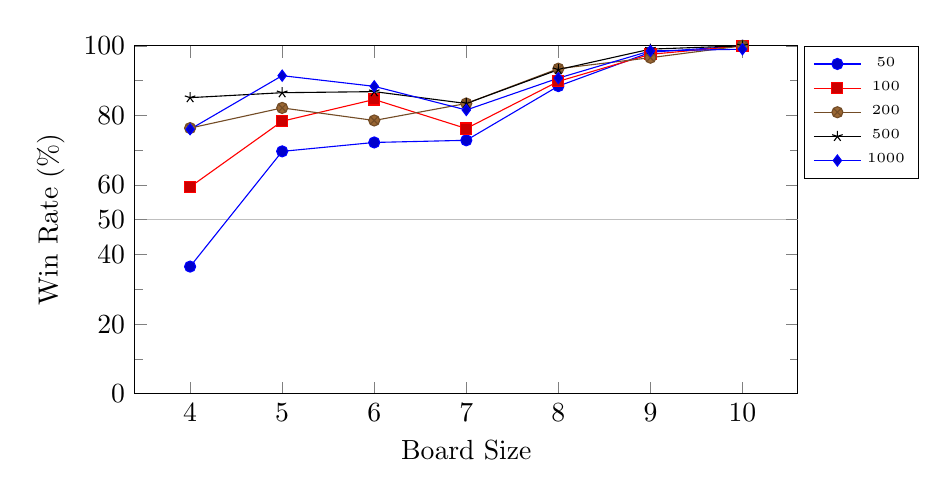
\begin{tikzpicture}
\begin{axis}[
	xlabel=Board Size,
	ylabel=Win Rate (\%),
	xtick={4,5,6,7,8,9,10},
	ymin=0, ymax=100,
	minor y tick num=1,
	extra y ticks={50},
	extra y tick style={grid=major},
]
\addplot coordinates { (4,36.54) (5,69.66) (6,72.22) (7,72.84) (8,88.42) (9,98.15) (10,100.00) }; \addlegendentry{   50}
\addplot coordinates { (4,59.43) (5,78.33) (6,84.57) (7,76.22) (8,89.78) (9,97.55) (10,100.00) }; \addlegendentry{  100}
\addplot coordinates { (4,76.35) (5,82.15) (6,78.54) (7,83.42) (8,93.43) (9,96.58) (10,100.00) }; \addlegendentry{  200}
\addplot coordinates { (4,85.10) (5,86.52) (6,86.83) (7,83.42) (8,93.15) (9,99.05) (10,100.00) }; \addlegendentry{  500}
\addplot coordinates { (4,76.02) (5,91.42) (6,88.35) (7,81.55) (8,90.71) (9,98.54) (10,99.02) }; \addlegendentry{ 1000}
\end{axis}
\end{tikzpicture}
	\caption{Rave vs UCT Baseline}
	\label{fig:ravegraph}
\end{figure}
\end{frame}


\begin{frame}{Proof Backups}
\begin{figure}
	\centering
	\begin{HavannahBoard}[board size=4,coordinate style=classical,show coordinates=false]
%	\HGame{b1,d2,a2,e4}
	\HStoneGroup[color=white]{b1,a2}
	\HStoneGroup[color=black]{d2,e4}
	\end{HavannahBoard}
	\caption{Early Position Solvable by MCTS in 1 Minute, white to play}
	\label{fig:lorentzproof}
\end{figure}
\end{frame}

\begin{frame}{Proof Backups}
\begin{figure}
\centering
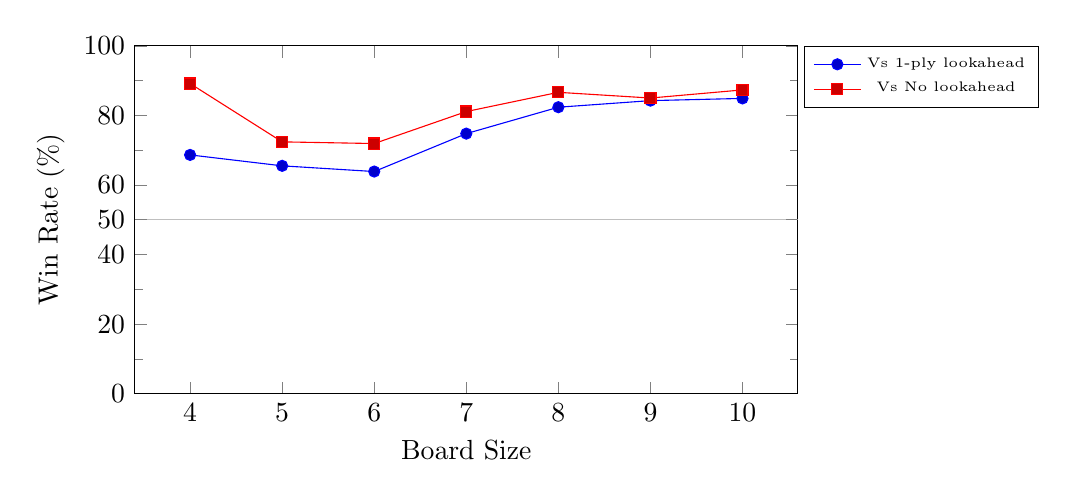
\begin{tikzpicture}
\begin{axis}[
	xlabel=Board Size,
	ylabel=Win Rate (\%),
	xtick={4,5,6,7,8,9,10},
	ymin=0, ymax=100,
	minor y tick num=1,
	extra y ticks={50},
	extra y tick style={grid=major},
]
\addplot coordinates { (4,68.64) (5,65.5) (6,63.86) (7,74.76) (8,82.35) (9,84.24) (10,84.88) }; \addlegendentry{Vs 1-ply lookahead}
\addplot coordinates { (4,89.15) (5,72.39) (6,71.91) (7,81.1) (8,86.63) (9,84.99) (10,87.32) }; \addlegendentry{Vs No lookahead}

%\addplot coordinates { (4,31.36) (5,34.50) (6,36.14) (7,25.24) (8,17.65) (9,15.76) (10,15.12) }; \addlegendentry{One ply}
%\addplot coordinates { (4,10.85) (5,27.61) (6,28.09) (7,18.90) (8,13.37) (9,15.01) (10,12.68) }; \addlegendentry{Disabled}
\end{axis}
\end{tikzpicture}
	\caption{RAVE Baseline with 2-ply lookahead during expansion vs 1-ply lookahead and no lookahead}
	\label{fig:proofbackups}
\end{figure}
\end{frame}


\begin{frame}{Multiple Rollouts}
%\only<1>{
\begin{table}
	\centering
	\begin{tabular}{l|rrrrr}
		             & Iterations & Descent & Expansion & Rollout & Back-prop \\ \hline
		UCT size 5   & 296136 & 33.6\% & 12.0\% & 48.4\% &  5.9\% \\
		UCT size 10  & 102192 & 24.8\% & 11.3\% & 62.0\% &  2.0\% \\
		RAVE size 5  & 148713 & 45.1\% &  7.3\% & 22.2\% & 25.4\% \\
		RAVE size 10 &  41713 & 42.9\% &  4.8\% & 24.3\% & 28.0\% \\
	\end{tabular}
	\caption{Time Used by MCTS Phase with 1 Rollout per Simulation}
	\label{tab:phasetime}
\end{table}
%}
\only<2>{
\begin{table}
	\centering
	\begin{tabular}{l|rrrrr}
		             & Iterations & Descent & Expansion & Rollout & Back-prop \\ \hline
		UCT size 5   & 201408 & 22.9\% & 7.0\% & 66.1\% &  4.0\% \\
		UCT size 10  &  66945 & 16.3\% & 3.5\% & 78.9\% &  1.3\% \\
		RAVE size 5  & 115704 & 34.7\% & 6.0\% & 32.6\% & 26.6\% \\
		RAVE size 10 &  31962 & 29.4\% & 4.0\% & 37.1\% & 29.6\% \\
	\end{tabular}
	\caption{Time Used by MCTS Phase Using 2 Rollouts per Simulation}
	\label{tab:phasetime2}
\end{table}
}
\only<3>{
\begin{table}
	\centering
	\begin{tabular}{l|rrrrr}
		             & Iterations & Descent & Expansion & Rollout & Back-prop \\ \hline
		UCT size 5   & 58786 &  6.5\% & 1.4\% & 91.0\% &  1.1\% \\
		UCT size 10  & 16616 &  3.9\% & 0.4\% & 95.4\% &  0.3\% \\
		RAVE size 5  & 49131 & 14.8\% & 3.4\% & 65.6\% & 16.2\% \\
		RAVE size 10 & 12232 & 10.7\% & 1.9\% & 71.1\% & 16.3\% \\
	\end{tabular}
	\caption{Time Used by MCTS Phase Using 10 Rollouts per Simulation}
	\label{tab:phasetime10}
\end{table}
}
\end{frame}

\begin{frame}{Multiple Rollouts}
\begin{figure}
	\centering
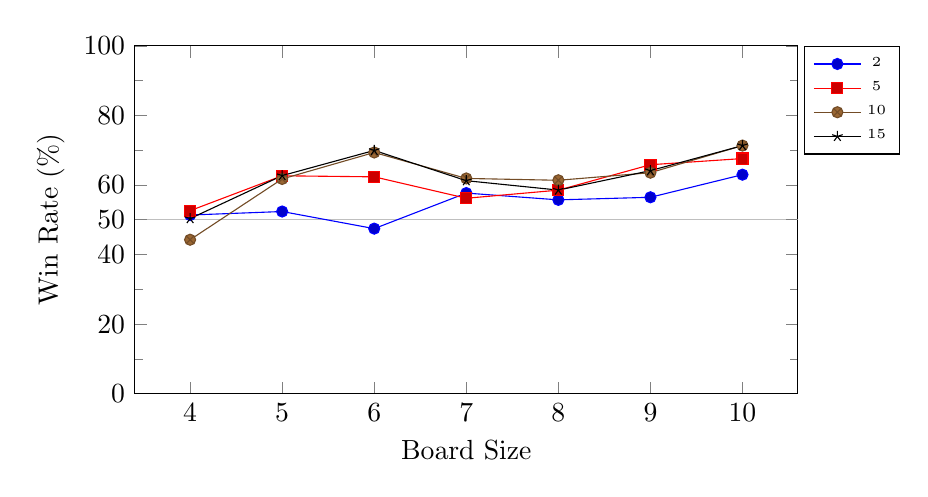
\begin{tikzpicture}
\begin{axis}[
	xlabel=Board Size,
	ylabel=Win Rate (\%),
	xtick={4,5,6,7,8,9,10},
	ymin=0, ymax=100,
	minor y tick num=1,
	extra y ticks={50},
	extra y tick style={grid=major},
]
\addplot coordinates { (4,51.36) (5,52.37) (6,47.45) (7,57.67) (8,55.72) (9,56.46) (10,62.96) }; \addlegendentry{ 2}
%\addplot coordinates { (4,50.62) (5,60.59) (6,54.13) (7,53.38) (8,58.92) (9,58.04) (10,65.88) }; \addlegendentry{ 3}
%\addplot coordinates { (4,51.19) (5,57.16) (6,55.11) (7,56.79) (8,59.25) (9,60.49) (10,70.09) }; \addlegendentry{ 4}
\addplot coordinates { (4,52.61) (5,62.64) (6,62.34) (7,56.18) (8,58.51) (9,65.82) (10,67.59) }; \addlegendentry{ 5}
%\addplot coordinates { (4,49.77) (5,55.93) (6,60.85) (7,56.40) (8,60.65) (9,59.08) (10,73.29) }; \addlegendentry{ 6}
%\addplot coordinates { (4,49.94) (5,59.04) (6,54.70) (7,52.52) (8,57.14) (9,66.13) (10,68.75) }; \addlegendentry{ 7}
%\addplot coordinates { (4,53.40) (5,59.93) (6,67.23) (7,55.61) (8,60.16) (9,68.39) (10,71.20) }; \addlegendentry{ 8}
%\addplot coordinates { (4,49.89) (5,62.83) (6,53.83) (7,59.96) (8,58.12) (9,68.94) (10,70.44) }; \addlegendentry{ 9}
\addplot coordinates { (4,44.26) (5,61.73) (6,69.34) (7,61.88) (8,61.35) (9,63.53) (10,71.33) }; \addlegendentry{10}
%\addplot coordinates { (4,48.01) (5,68.65) (6,66.78) (7,54.74) (8,61.71) (9,63.70) (10,68.99) }; \addlegendentry{12}
\addplot coordinates { (4,50.34) (5,62.69) (6,69.93) (7,61.23) (8,58.53) (9,64.12) (10,71.31) }; \addlegendentry{15}
%\addplot coordinates { (4,47.67) (5,64.08) (6,56.59) (7,53.61) (8,62.60) (9,67.85) (10,77.37) }; \addlegendentry{20}
\end{axis}
\end{tikzpicture}
	\caption[Multiple Rollouts]{Multiple Rollouts per Simulation Against Baseline RAVE Player}
	\label{fig:multirollouts}
\end{figure}
\end{frame}


\subsection{Knowledge}

\begin{frame}{Maintain Virtual Connections}
\begin{figure}
	\centering
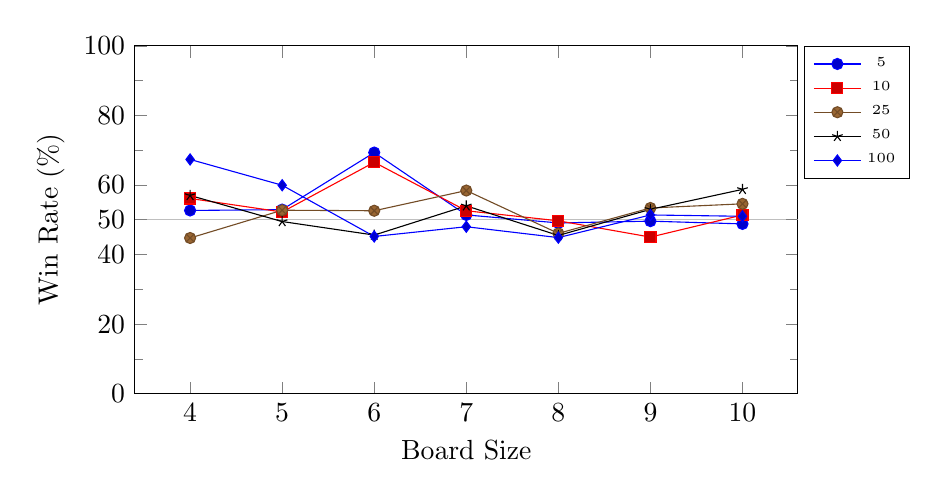
\begin{tikzpicture}
\begin{axis}[
	xlabel=Board Size,
	ylabel=Win Rate (\%),
	xtick={4,5,6,7,8,9,10},
	ymin=0, ymax=100,
	minor y tick num=1,
	extra y ticks={50},
	extra y tick style={grid=major},
]
\addplot coordinates { (4,52.67) (5,52.92) (6,69.32) (7,51.39) (8,49.09) (9,49.60) (10,48.81) }; \addlegendentry{  5}
\addplot coordinates { (4,56.12) (5,52.23) (6,66.53) (7,52.59) (8,49.70) (9,45.02) (10,51.37) }; \addlegendentry{ 10}
\addplot coordinates { (4,44.76) (5,52.74) (6,52.59) (7,58.40) (8,46.09) (9,53.39) (10,54.58) }; \addlegendentry{ 25}
\addplot coordinates { (4,56.99) (5,49.49) (6,45.60) (7,54.00) (8,45.49) (9,52.99) (10,58.73) }; \addlegendentry{ 50}
\addplot coordinates { (4,67.34) (5,59.92) (6,45.20) (7,48.00) (8,44.87) (9,51.38) (10,51.00) }; \addlegendentry{100}
\end{axis}
\end{tikzpicture}
	\caption[Maintain Virtual Connection Bonus]{Maintain Virtual Connection Bonus Against Baseline RAVE Player}
	\label{fig:maintainvc}
\end{figure}
\end{frame}

\begin{frame}{Locality}
\begin{figure}
	\centering
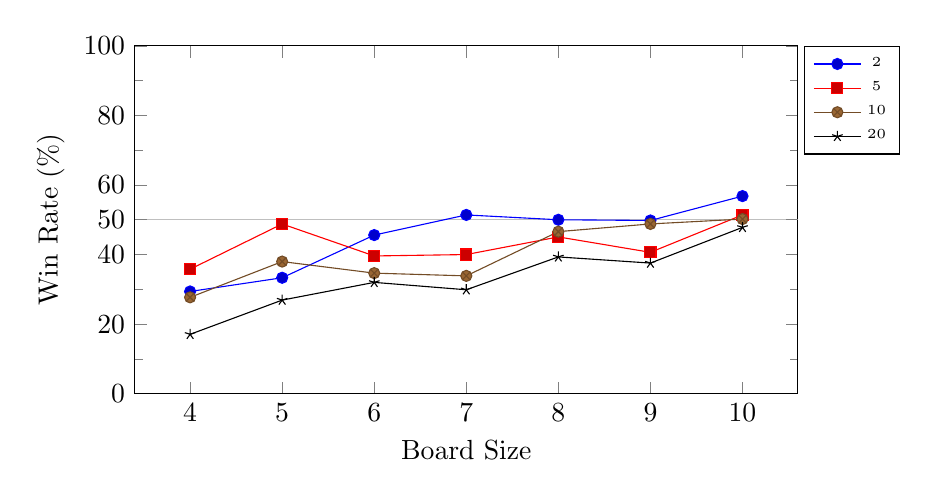
\begin{tikzpicture}
\begin{axis}[
	xlabel=Board Size,
	ylabel=Win Rate (\%),
	xtick={4,5,6,7,8,9,10},
	ymin=0, ymax=100,
	minor y tick num=1,
	extra y ticks={50},
	extra y tick style={grid=major},
]
%\addplot coordinates { (4,40.86) (5,37.30) (6,34.00) (7,48.06) (8,57.03) (9,49.00) (10,42.74) }; \addlegendentry{ 1}
\addplot coordinates { (4,29.39) (5,33.33) (6,45.60) (7,51.39) (8,50.00) (9,49.80) (10,56.80) }; \addlegendentry{ 2}
\addplot coordinates { (4,35.79) (5,48.79) (6,39.60) (7,40.00) (8,45.07) (9,40.64) (10,51.39) }; \addlegendentry{ 5}
\addplot coordinates { (4,27.70) (5,37.98) (6,34.66) (7,33.87) (8,46.59) (9,48.80) (10,50.20) }; \addlegendentry{10}
\addplot coordinates { (4,17.07) (5,26.91) (6,32.00) (7,29.88) (8,39.32) (9,37.55) (10,47.81) }; \addlegendentry{20}
%\addplot coordinates { (4,1.21) (5,18.88) (6,26.98) (7,39.04) (8,31.53) (9,31.47) (10,35.46) }; \addlegendentry{50}
\end{axis}
\end{tikzpicture}
	\caption[Locality Bonus, Any Stones]{Locality Bonus for Playing Near Existing Stones of any Colour Against Baseline RAVE Player}
	\label{fig:localityany}
\end{figure}
\end{frame}

\begin{frame}{Locality}
\begin{figure}
	\centering
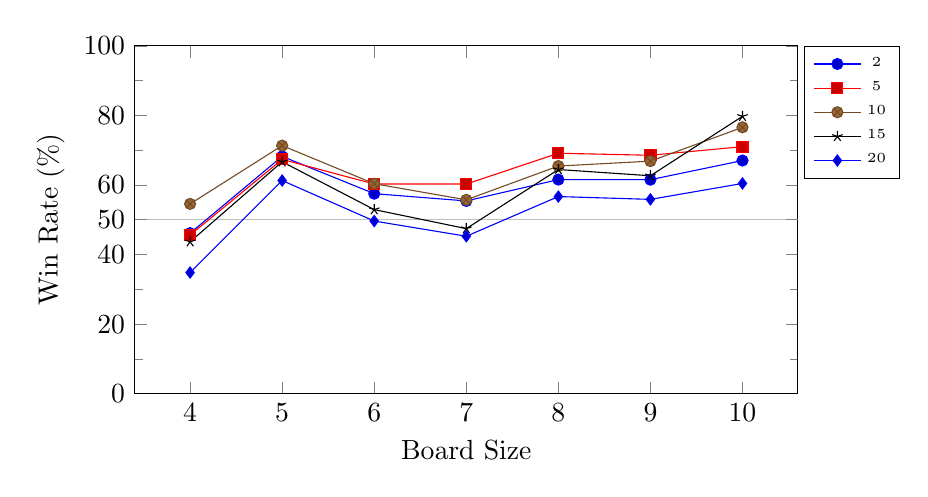
\begin{tikzpicture}
\begin{axis}[
	xlabel=Board Size,
	ylabel=Win Rate (\%),
	xtick={4,5,6,7,8,9,10},
	ymin=0, ymax=100,
	minor y tick num=1,
	extra y ticks={50},
	extra y tick style={grid=major},
]
%\addplot coordinates { (4,55.41) (5,60.06) (6,57.34) (7,46.53) (8,57.76) (9,57.96) (10,61.31) }; \addlegendentry{ 1}
\addplot coordinates { (4,46.15) (5,68.22) (6,57.50) (7,55.41) (8,61.54) (9,61.52) (10,67.02) }; \addlegendentry{ 2}
\addplot coordinates { (4,45.61) (5,67.35) (6,60.27) (7,60.27) (8,69.12) (9,68.54) (10,71.01) }; \addlegendentry{ 5}
\addplot coordinates { (4,54.56) (5,71.32) (6,60.36) (7,55.73) (8,65.44) (9,66.85) (10,76.57) }; \addlegendentry{10}
\addplot coordinates { (4,43.67) (5,66.67) (6,52.92) (7,47.45) (8,64.44) (9,62.65) (10,79.73) }; \addlegendentry{15}
\addplot coordinates { (4,34.83) (5,61.28) (6,49.63) (7,45.26) (8,56.67) (9,55.86) (10,60.44) }; \addlegendentry{20}
%\addplot coordinates { (4,20.90) (5,53.53) (6,43.90) (7,45.20) (8,42.18) (9,47.95) (10,60.00) }; \addlegendentry{50}
\end{axis}
\end{tikzpicture}
	\caption[Locality Bonus, Own Stones]{Locality Bonus for Playing Near Stones of the Same Colour Against Baseline RAVE Player}
	\label{fig:localitysides}
\end{figure}
\end{frame}


\begin{frame}{Local Reply}
\begin{figure}
	\centering
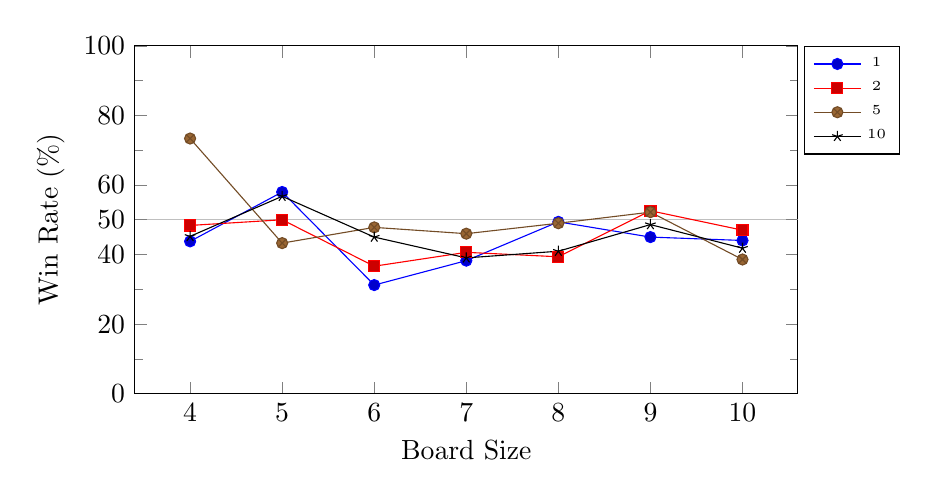
\begin{tikzpicture}
\begin{axis}[
	xlabel=Board Size,
	ylabel=Win Rate (\%),
	xtick={4,5,6,7,8,9,10},
	ymin=0, ymax=100,
	minor y tick num=1,
	extra y ticks={50},
	extra y tick style={grid=major},
]
\addplot coordinates { (4,43.79) (5,57.98) (6,31.23) (7,38.25) (8,49.40) (9,45.02) (10,44.05) }; \addlegendentry{ 1}
\addplot coordinates { (4,48.37) (5,50.00) (6,36.65) (7,40.64) (8,39.36) (9,52.59) (10,47.01) }; \addlegendentry{ 2}
\addplot coordinates { (4,73.35) (5,43.29) (6,47.81) (7,46.00) (8,49.00) (9,52.19) (10,38.58) }; \addlegendentry{ 5}
\addplot coordinates { (4,45.23) (5,56.74) (6,45.02) (7,39.04) (8,40.96) (9,48.61) (10,41.83) }; \addlegendentry{10}
%\addplot coordinates { (4,37.25) (5,31.99) (6,41.20) (7,46.40) (8,38.52) (9,46.83) (10,44.22) }; \addlegendentry{20}
%\addplot coordinates { (4,19.55) (5,27.31) (6,33.33) (7,30.80) (8,19.24) (9,25.69) (10,23.92) }; \addlegendentry{50}
\end{axis}
\end{tikzpicture}
	\caption[Local Reply Bonus]{Local Reply Bonus for Playing Near the Opponent's Last Move Against Baseline RAVE Player}
	\label{fig:localreply}
\end{figure}
\end{frame}

\begin{frame}{Edge Connectivity}
\begin{figure}
	\centering
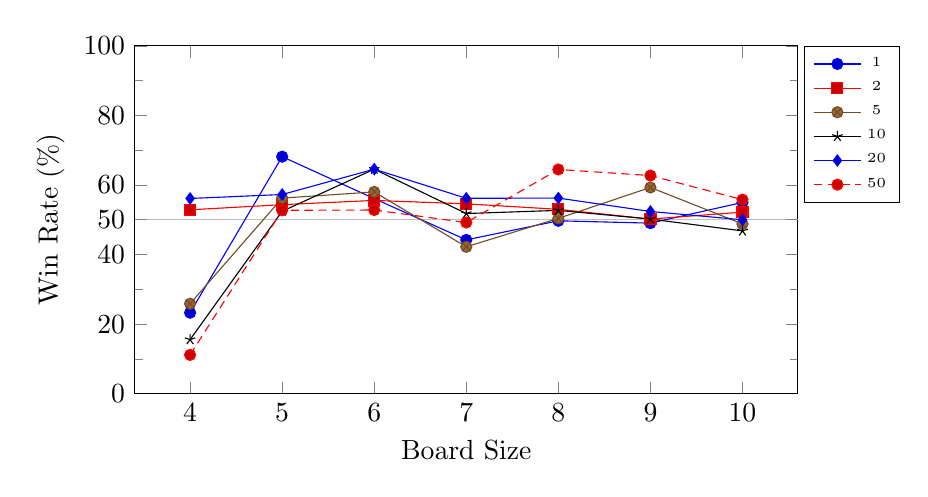
\begin{tikzpicture}
\begin{axis}[
	xlabel=Board Size,
	ylabel=Win Rate (\%),
	xtick={4,5,6,7,8,9,10},
	ymin=0, ymax=100,
	minor y tick num=1,
	extra y ticks={50},
	extra y tick style={grid=major},
]
%\addplot coordinates { (4,28.99) (5,54.56) (6,50.20) (7,48.39) (8,58.59) (9,56.05) (10,51.42) }; \addlegendentry{ 0.2}
%\addplot coordinates { (4,31.82) (5,58.78) (6,62.10) (7,56.27) (8,55.56) (9,56.05) (10,47.98) }; \addlegendentry{ 0.5}
\addplot coordinates { (4,23.28) (5,68.14) (6,56.08) (7,44.22) (8,49.70) (9,49.03) (10,54.98) }; \addlegendentry{ 1}
\addplot coordinates { (4,52.86) (5,54.34) (6,55.56) (7,54.58) (8,53.00) (9,50.20) (10,52.19) }; \addlegendentry{ 2}
\addplot coordinates { (4,25.87) (5,56.23) (6,58.00) (7,42.23) (8,50.40) (9,59.29) (10,48.81) }; \addlegendentry{ 5}
\addplot coordinates { (4,15.56) (5,52.44) (6,64.54) (7,51.79) (8,52.70) (9,50.20) (10,46.80) }; \addlegendentry{10}
\addplot coordinates { (4,56.12) (5,57.26) (6,64.54) (7,56.17) (8,56.23) (9,52.38) (10,50.00) }; \addlegendentry{20}
\addplot coordinates { (4,11.16) (5,52.72) (6,52.80) (7,49.20) (8,64.46) (9,62.70) (10,55.78) }; \addlegendentry{50}
\end{axis}
\end{tikzpicture}
	\caption[Edge Connectivity Bonus]{Edge Connectivity Bonus for Playing Near Groups that are Connected to an Edge or Corner Against Baseline RAVE Player}
	\label{fig:connectivity}
\end{figure}
\end{frame}

\begin{frame}{Group Size}
\begin{figure}
	\centering
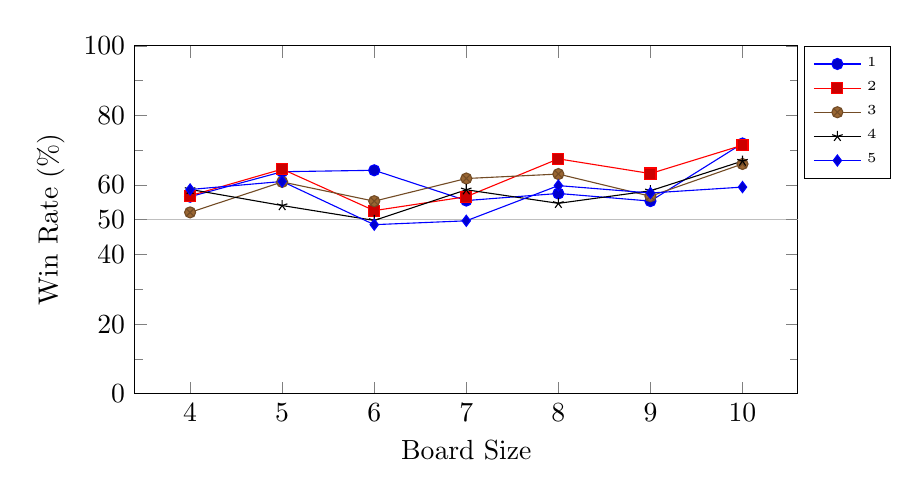
\begin{tikzpicture}
\begin{axis}[
	xlabel=Board Size,
	ylabel=Win Rate (\%),
	xtick={4,5,6,7,8,9,10},
	ymin=0, ymax=100,
	minor y tick num=1,
	extra y ticks={50},
	extra y tick style={grid=major},
]
\addplot coordinates { (4,56.63) (5,63.81) (6,64.22) (7,55.52) (8,57.56) (9,55.37) (10,71.92) }; \addlegendentry{  1}
\addplot coordinates { (4,56.92) (5,64.56) (6,52.63) (7,56.63) (8,67.51) (9,63.28) (10,71.43) }; \addlegendentry{  2}
\addplot coordinates { (4,52.12) (5,60.87) (6,55.34) (7,61.86) (8,63.14) (9,56.76) (10,66.04) }; \addlegendentry{  3}
\addplot coordinates { (4,58.73) (5,54.09) (6,49.81) (7,58.62) (8,54.72) (9,58.33) (10,66.87) }; \addlegendentry{  4}
\addplot coordinates { (4,58.70) (5,61.01) (6,48.59) (7,49.70) (8,59.82) (9,57.69) (10,59.39) }; \addlegendentry{  5}
%\addplot coordinates { (4,59.68) (5,61.13) (6,47.77) (7,55.72) (8,47.51) (9,45.58) (10,49.11) }; \addlegendentry{ 10}
%\addplot coordinates { (4,50.47) (5,42.84) (6,44.48) (7,50.43) (8,42.64) (9,44.92) (10,39.32) }; \addlegendentry{ 20}
%\addplot coordinates { (4,33.44) (5,42.65) (6,33.13) (7,40.36) (8,34.10) (9,28.88) (10,31.33) }; \addlegendentry{ 50}
%\addplot coordinates { (4,21.80) (5,30.79) (6,37.54) (7,30.45) (8,29.04) (9,19.21) (10,14.63) }; \addlegendentry{100}
%\addplot coordinates { (4,13.02) (5,20.64) (6,21.43) (7,14.37) (8,18.54) (9,9.71) (10,10.61) }; \addlegendentry{200}
\end{axis}
\end{tikzpicture}
	\caption[Group Size Bonus]{Group Size Bonus for Playing Near or Forming Big Groups Against Baseline RAVE Player}
	\label{fig:groupsize}
\end{figure}
\end{frame}

\begin{frame}{Distance to Win}
\only<1>{
\begin{figure}
	\centering
	\begin{HavannahBoard}[board size=4,coordinate style=classical,show coordinates=false]
	\HGame[numbered moves=false]{a4,g4,a1,b3,g7,d1,d7,f3,e2,d2}
	\HStoneGroup[color=light gray,label=1]{}
	\HStoneGroup[color=light gray,label=2]{a2,a3,b5,c6,e7,f7}
	\HStoneGroup[color=light gray,label=3]{b1,b2,b4,c5,d6,e6,f6,g6}
	\HStoneGroup[color=light gray,label=4]{c3,c4,d5,e5}
	\HStoneGroup[color=light gray,label=5]{c1,c2,d4,f5,g5}
	\HStoneGroup[color=light gray,label=6]{d3,e3,e4,f4}
	\end{HavannahBoard}
	\caption{Distance to a Win for White}
\end{figure}
}
\only<2>{
\begin{figure}
	\centering
	\begin{HavannahBoard}[board size=4,coordinate style=classical,show coordinates=false]
	\HGame[numbered moves=false]{a4,g4,a1,b3,g7,d1,d7,f3,e2,d2}
	\HStoneGroup[color=light gray,label=1]{e3}
	\HStoneGroup[color=light gray,label=2]{c1,c2,d3,f4,g5}
	\HStoneGroup[color=light gray,label=3]{e4}
	\HStoneGroup[color=light gray,label=4]{b1,b2,c3,d4,f5,g6}
	\HStoneGroup[color=light gray,label=5]{a2,a3,b4,e5,f6}
	\HStoneGroup[color=light gray,label=6]{b5,c4,c5,c6,d5,d6,e6,e7,f7}
	\end{HavannahBoard}
	\caption{Distance to a Win for Black}
\end{figure}
}
\only<3>{
\begin{figure}
	\centering
	\begin{HavannahBoard}[board size=4,coordinate style=classical,show coordinates=false]
	\HGame[numbered moves=false]{a4,g4,a1,b3,g7,d1,d7,f3,e2,d2}
	\HStoneGroup[color=light gray,label=1]{e3}
	\HStoneGroup[color=light gray,label=2]{a2,a3,b5,c1,c2,c6,d3,e7,f4,f7,g5}
	\HStoneGroup[color=light gray,label=3]{b1,b2,b4,c5,d6,e4,e6,f6,g6}
	\HStoneGroup[color=light gray,label=4]{c3,c4,d4,d5,e5,f5}
	\end{HavannahBoard}
	\caption{Distance to a Win, Minimum of White and Black}
\end{figure}
}
\end{frame}

\begin{frame}{Distance to Win, Minimum}
\begin{figure}
	\centering
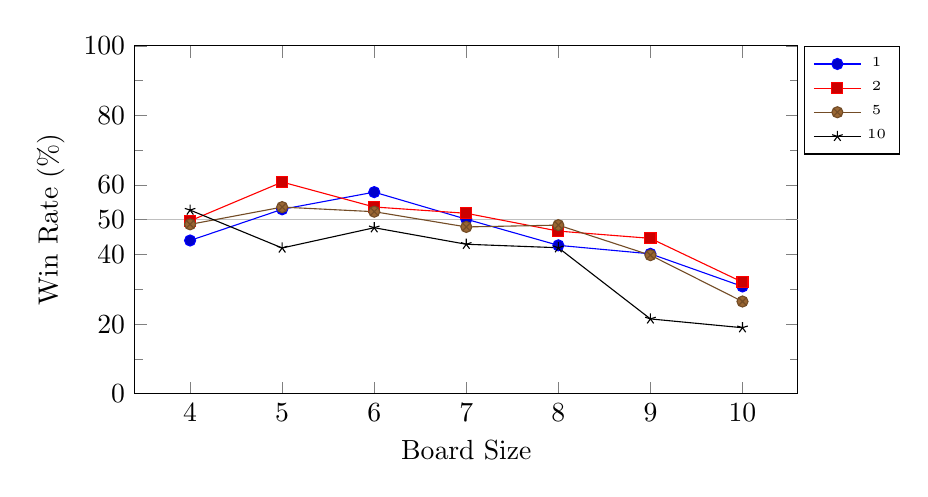
\begin{tikzpicture}
\begin{axis}[
	xlabel=Board Size,
	ylabel=Win Rate (\%),
	xtick={4,5,6,7,8,9,10},
	ymin=0, ymax=100,
	minor y tick num=1,
	extra y ticks={50},
	extra y tick style={grid=major},
]
\addplot coordinates { (4,44.04) (5,53.01) (6,57.94) (7,50.16) (8,42.65) (9,40.21) (10,30.83) }; \addlegendentry{  1}
\addplot coordinates { (4,49.69) (5,60.84) (6,53.67) (7,51.86) (8,46.74) (9,44.66) (10,32.06) }; \addlegendentry{  2}
%\addplot coordinates { (4,50.54) (5,59.89) (6,54.69) (7,52.77) (8,49.39) (9,39.27) (10,30.13) }; \addlegendentry{  3}
%\addplot coordinates { (4,50.31) (5,57.19) (6,58.67) (7,51.14) (8,48.53) (9,38.66) (10,29.20) }; \addlegendentry{  4}
\addplot coordinates { (4,48.68) (5,53.64) (6,52.32) (7,47.94) (8,48.46) (9,39.82) (10,26.50) }; \addlegendentry{  5}
\addplot coordinates { (4,52.78) (5,41.89) (6,47.71) (7,42.96) (8,41.96) (9,21.50) (10,18.97) }; \addlegendentry{ 10}
%\addplot coordinates { (4,32.22) (5,32.35) (6,37.18) (7,35.24) (8,30.69) (9,18.75) (10,17.44) }; \addlegendentry{ 20}
%\addplot coordinates { (4,10.00) (5,23.33) (6,19.67) (7,25.26) (8,16.30) (9,8.70) (10,6.14) }; \addlegendentry{ 50}
%\addplot coordinates { (4,6.56) (5,13.64) (6,15.19) (7,11.32) (8,12.93) (9,15.79) (10,12.50) }; \addlegendentry{100}
%\addplot coordinates { (4,2.27) (5,10.77) (6,12.68) (7,5.75) (8,16.87) (9,23.29) (10,10.71) }; \addlegendentry{200}
\end{axis}
\end{tikzpicture}
	\caption[Minimum Distance to Win Bonus]{Minimum Distance to Win Bonus Against Baseline RAVE Player}
	\label{fig:distancetogether}
\end{figure}
\end{frame}

\begin{frame}{Distance to Win, Own Side}
\begin{figure}
	\centering
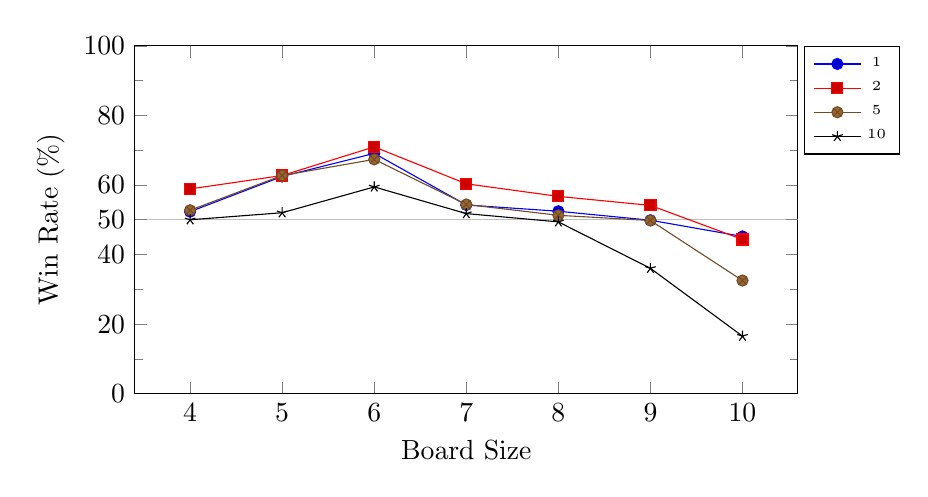
\begin{tikzpicture}
\begin{axis}[
	xlabel=Board Size,
	ylabel=Win Rate (\%),
	xtick={4,5,6,7,8,9,10},
	ymin=0, ymax=100,
	minor y tick num=1,
	extra y ticks={50},
	extra y tick style={grid=major},
]
\addplot coordinates { (4,52.33) (5,62.45) (6,69.08) (7,54.25) (8,52.45) (9,49.87) (10,45.21) }; \addlegendentry{ 1}
\addplot coordinates { (4,58.86) (5,62.72) (6,70.95) (7,60.34) (8,56.72) (9,54.13) (10,44.33) }; \addlegendentry{ 2}
%\addplot coordinates { (4,54.02) (5,62.36) (6,63.20) (7,58.46) (8,57.03) (9,53.03) (10,42.02) }; \addlegendentry{ 3}
%\addplot coordinates { (4,44.30) (5,57.25) (6,61.73) (7,59.86) (8,58.20) (9,53.98) (10,41.07) }; \addlegendentry{ 4}
\addplot coordinates { (4,52.74) (5,62.72) (6,67.36) (7,54.39) (8,51.28) (9,49.79) (10,32.53) }; \addlegendentry{ 5}
\addplot coordinates { (4,50.00) (5,52.02) (6,59.44) (7,51.77) (8,49.39) (9,36.04) (10,16.55) }; \addlegendentry{10}
\end{axis}
\end{tikzpicture}
	\caption[Own Minimum Distance to Win]{Own Minimum Distance to Win Bonus Against Baseline RAVE Player}
	\label{fig:distancesides}
\end{figure}
\end{frame}


\subsection{Rollout Policy}

\begin{frame}{Mate-in-one}
\begin{figure}
	\centering
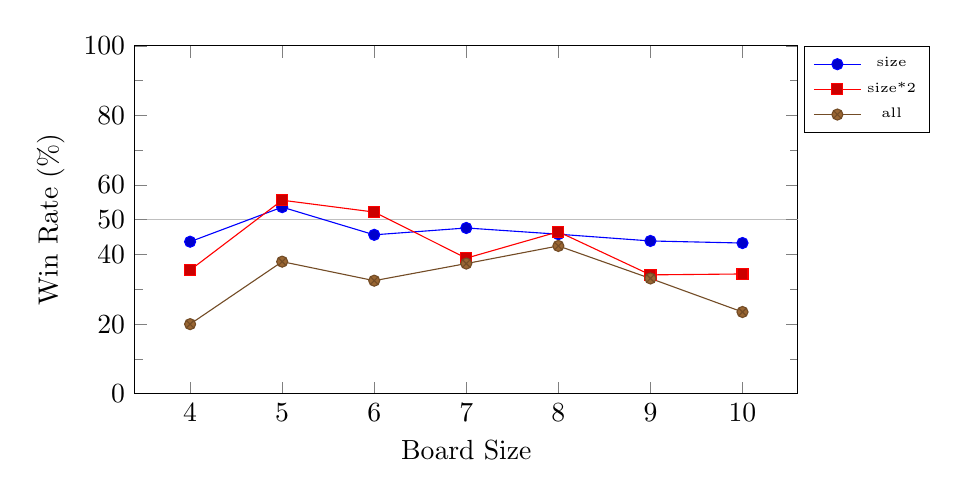
\begin{tikzpicture}
\begin{axis}[
	xlabel=Board Size,
	ylabel=Win Rate (\%),
	xtick={4,5,6,7,8,9,10},
	ymin=0, ymax=100,
	minor y tick num=1,
	extra y ticks={50},
	extra y tick style={grid=major},
]
%\addplot coordinates { (4,54.26) (5,47.92) (6,43.78) (7,49.27) (8,51.75) (9,46.91) (10,50.58) }; \addlegendentry{2}
%\addplot coordinates { (4,48.75) (5,57.66) (6,53.06) (7,49.32) (8,44.49) (9,44.85) (10,48.77) }; \addlegendentry{5}
%\addplot coordinates { (4,27.78) (5,54.42) (6,48.87) (7,44.27) (8,40.97) (9,45.27) (10,46.71) }; \addlegendentry{10}
\addplot coordinates { (4,43.69) (5,53.63) (6,45.67) (7,47.64) (8,45.85) (9,43.91) (10,43.31) }; \addlegendentry{size}
\addplot coordinates { (4,35.53) (5,55.62) (6,52.21) (7,38.96) (8,46.55) (9,34.16) (10,34.42) }; \addlegendentry{size*2}
\addplot coordinates { (4,20.00) (5,37.96) (6,32.49) (7,37.41) (8,42.48) (9,33.13) (10,23.49) }; \addlegendentry{all}
\end{axis}
\end{tikzpicture}
	\caption{Mate-in-one Checking Against Baseline RAVE Player With 5 Seconds per Move}
	\label{fig:mateinone}
\end{figure}
\end{frame}

\begin{frame}{Maintain Virtual Connections}
\begin{figure}
	\centering
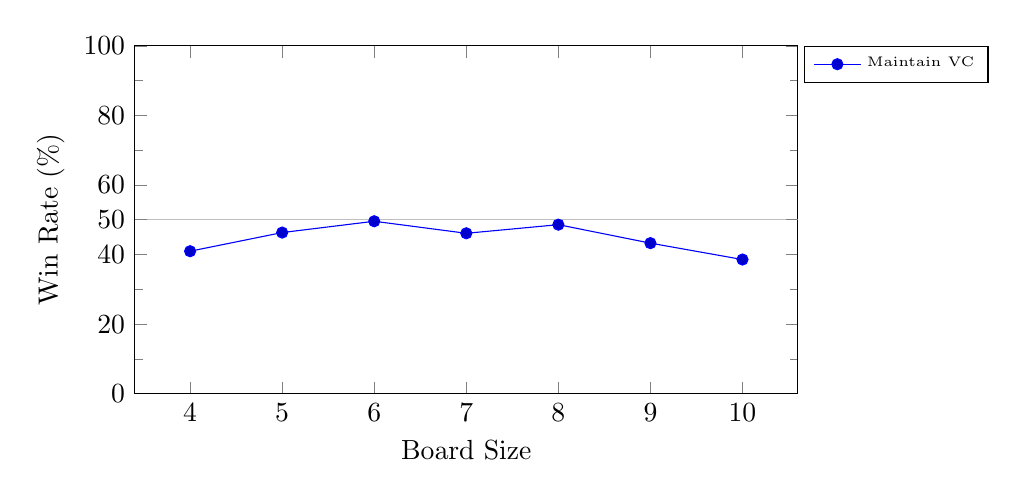
\begin{tikzpicture}
\begin{axis}[
	xlabel=Board Size,
	ylabel=Win Rate (\%),
	xtick={4,5,6,7,8,9,10},
	ymin=0, ymax=100,
	minor y tick num=1,
	extra y ticks={50},
	extra y tick style={grid=major},
]
\addplot coordinates { (4,40.96) (5,46.32) (6,49.57) (7,46.11) (8,48.59) (9,43.28) (10,38.57) }; \addlegendentry{Maintain VC}
\end{axis}
\end{tikzpicture}
	\caption{Maintain Virtual Connections in the Rollout Against Baseline RAVE Player}
	\label{fig:maintainvcrollout}
\end{figure}
\end{frame}

\begin{frame}{Last Good Reply}
\begin{figure}
	\centering
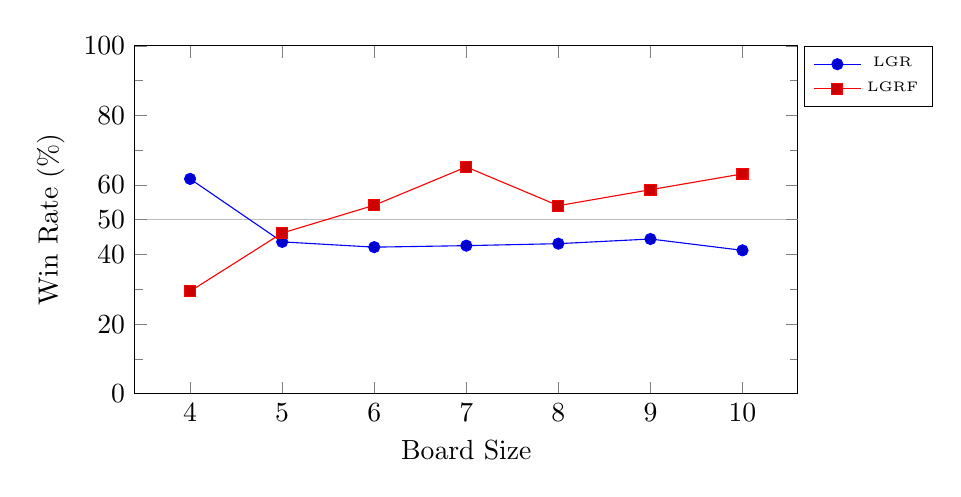
\begin{tikzpicture}
\begin{axis}[
	xlabel=Board Size,
	ylabel=Win Rate (\%),
	xtick={4,5,6,7,8,9,10},
	ymin=0, ymax=100,
	minor y tick num=1,
	extra y ticks={50},
	extra y tick style={grid=major},
]
\addplot coordinates { (4,61.75) (5,43.64) (6,42.13) (7,42.56) (8,43.13) (9,44.47) (10,41.21) }; \addlegendentry{LGR}
\addplot coordinates { (4,29.45) (5,46.19) (6,54.17) (7,65.18) (8,54.05) (9,58.64) (10,63.19) }; \addlegendentry{LGRF}
\end{axis}
\end{tikzpicture}
	\caption{Last Good Reply Against Baseline RAVE Player}
	\label{fig:lgr}
\end{figure}

\end{frame}

\begin{frame}{Ring Rule Variations}
\begin{table}
	\centering
	\begin{tabular}{l|rrr}
		Size & Fork & Bridge & Ring \\ \hline
		   4 & 4267 &   5177 &  543 \\
		   5 & 5111 &   2962 & 1926 \\
		   6 & 4471 &   1691 & 3838 \\
		   7 & 3536 &   1007 & 5457 \\
		   8 & 2266 &    460 & 7274 \\
		   9 & 1365 &    229 & 8406 \\
		   10 & 796 &    126 & 9078 \\
	\end{tabular}
	\caption{Number of Wins of Each Type by Board Size Given 10000 Simulations}
	\label{tab:wintypes}
\end{table}
\end{frame}

\begin{frame}{Ring Rule: Ignore all rings}
\begin{figure}
	\centering
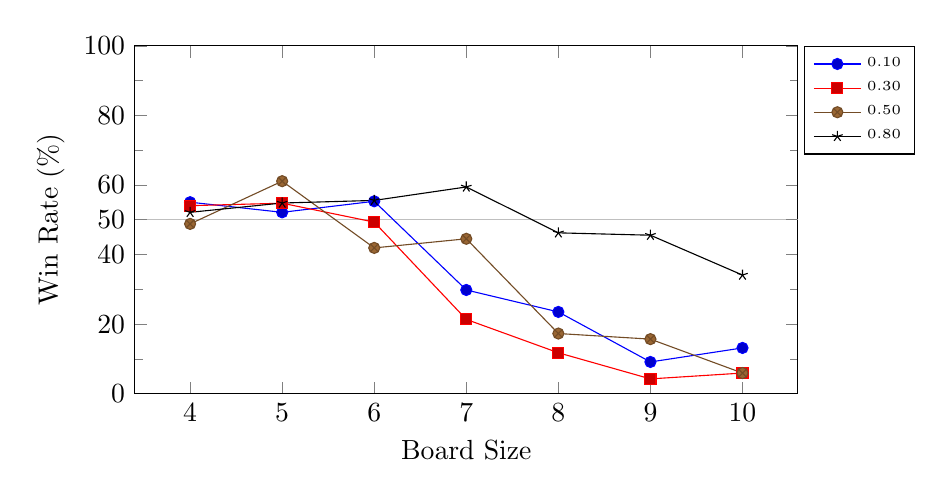
\begin{tikzpicture}
\begin{axis}[
	xlabel=Board Size,
	ylabel=Win Rate (\%),
	xtick={4,5,6,7,8,9,10},
	ymin=0, ymax=100,
	minor y tick num=1,
	extra y ticks={50},
	extra y tick style={grid=major},
]
%\addplot coordinates { (4,57.69) (5,53.65) (6,49.08) (7,29.83) (8,4.83) (9,5.26) (10,15.16) }; \addlegendentry{0.05}
\addplot coordinates { (4,55.05) (5,52.14) (6,55.31) (7,29.82) (8,23.51) (9,9.13) (10,13.16) }; \addlegendentry{0.10}
%\addplot coordinates { (4,55.47) (5,55.16) (6,56.65) (7,26.76) (8,8.33) (9,4.22) (10,12.45) }; \addlegendentry{0.20}
\addplot coordinates { (4,54.05) (5,54.76) (6,49.33) (7,21.36) (8,11.77) (9,4.26) (10,5.94) }; \addlegendentry{0.30}
\addplot coordinates { (4,48.81) (5,61.09) (6,41.91) (7,44.53) (8,17.30) (9,15.69) (10,5.94) }; \addlegendentry{0.50}
\addplot coordinates { (4,52.14) (5,54.81) (6,55.56) (7,59.43) (8,46.24) (9,45.56) (10,34.11) }; \addlegendentry{0.80}
\end{axis}
\end{tikzpicture}
	\caption{Ring Rule Ignore Rings Against Baseline RAVE Player}
	\label{fig:ringignore}
\end{figure}
\end{frame}

\begin{frame}{Ring Rule: Fixed depth}
\begin{table}
	\centering
	\begin{tabular}{l|rrr}
		Size & Fork   & Bridge &   Ring \\ \hline
		   4 &  29.56 &  26.34 &  28.00 \\
		   5 &  48.13 &  44.77 &  44.36 \\
		   6 &  71.66 &  68.01 &  65.07 \\
		   7 &  98.91 &  93.74 &  89.14 \\
		   8 & 131.29 & 126.29 & 116.38 \\
		   9 & 167.01 & 160.12 & 146.13 \\
		  10 & 206.35 & 196.88 & 177.64 \\
	\end{tabular}
	\caption{Average Number of Moves in a Rollout Before Each Victory Type}
	\label{tab:wintypedepth}
\end{table}
\end{frame}

\begin{frame}{Ring Rule: Fixed depth}
\begin{figure}
	\centering
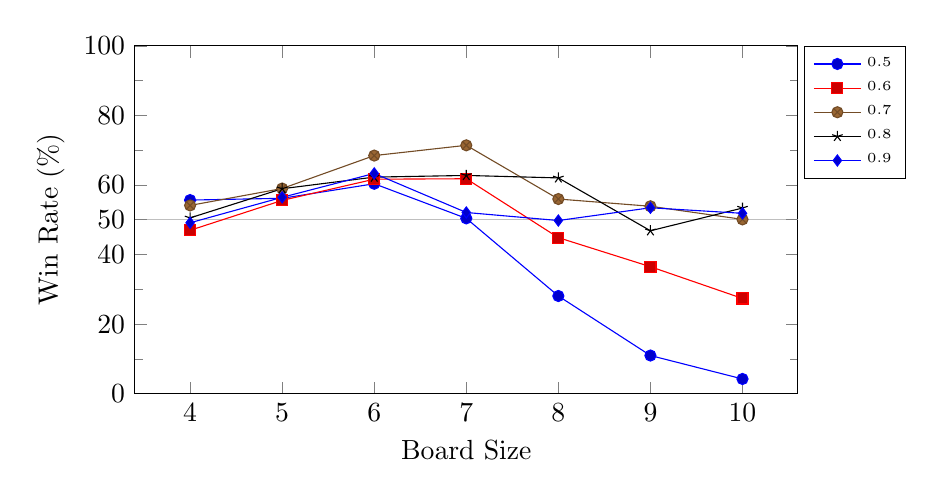
\begin{tikzpicture}
\begin{axis}[
	xlabel=Board Size,
	ylabel=Win Rate (\%),
	xtick={4,5,6,7,8,9,10},
	ymin=0, ymax=100,
	minor y tick num=1,
	extra y ticks={50},
	extra y tick style={grid=major},
]
%\addplot coordinates { (4,51.37) (5,51.77) (6,48.62) (7,30.49) (8,8.21) (9,2.99) (10,5.46) }; \addlegendentry{0.2}
%\addplot coordinates { (4,45.51) (5,55.66) (6,49.71) (7,32.30) (8,10.31) (9,4.23) (10,5.72) }; \addlegendentry{0.3}
%\addplot coordinates { (4,53.69) (5,50.77) (6,53.67) (7,37.78) (8,15.31) (9,3.96) (10,10.99) }; \addlegendentry{0.4}
\addplot coordinates { (4,55.66) (5,56.17) (6,60.35) (7,50.40) (8,28.09) (9,10.98) (10,4.24) }; \addlegendentry{0.5}
\addplot coordinates { (4,46.97) (5,55.57) (6,61.66) (7,61.79) (8,44.86) (9,36.51) (10,27.38) }; \addlegendentry{0.6}
\addplot coordinates { (4,54.12) (5,58.98) (6,68.45) (7,71.40) (8,55.96) (9,53.88) (10,50.11) }; \addlegendentry{0.7}
\addplot coordinates { (4,50.54) (5,58.92) (6,62.26) (7,62.74) (8,62.03) (9,46.84) (10,53.37) }; \addlegendentry{0.8}
\addplot coordinates { (4,49.13) (5,56.45) (6,63.32) (7,52.09) (8,49.78) (9,53.45) (10,51.85) }; \addlegendentry{0.9}

\end{axis}
\end{tikzpicture}
	\caption{Ring Rule Fixed Depth Against Baseline RAVE Player}
	\label{fig:ringdepth}
\end{figure}
\end{frame}

\begin{frame}{Ring Rule: Ring size}
\begin{figure}
	\centering
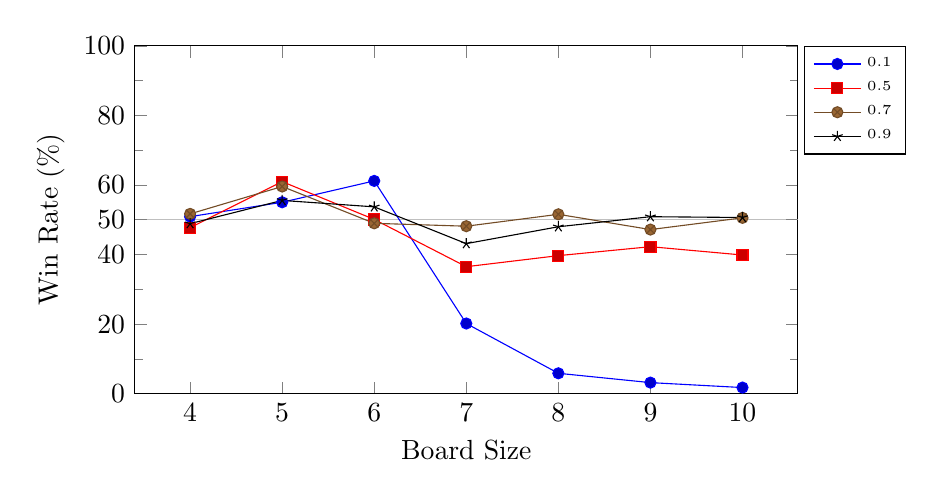
\begin{tikzpicture}
\begin{axis}[
	xlabel=Board Size,
	ylabel=Win Rate (\%),
	xtick={4,5,6,7,8,9,10},
	ymin=0, ymax=100,
	minor y tick num=1,
	extra y ticks={50},
	extra y tick style={grid=major},
]
\addplot coordinates { (4,50.90) (5,55.03) (6,61.17) (7,20.18) (8,5.87) (9,3.19) (10,1.77) }; \addlegendentry{0.1}
%\addplot coordinates { (4,50.00) (5,61.72) (6,51.25) (7,32.39) (8,19.07) (9,14.60) (10,10.09) }; \addlegendentry{0.2}
%\addplot coordinates { (4,49.77) (5,61.53) (6,48.34) (7,40.72) (8,30.29) (9,29.09) (10,23.42) }; \addlegendentry{0.3}
%\addplot coordinates { (4,48.70) (5,59.83) (6,48.68) (7,34.78) (8,34.75) (9,34.83) (10,34.55) }; \addlegendentry{0.4}
\addplot coordinates { (4,47.72) (5,60.96) (6,50.10) (7,36.51) (8,39.69) (9,42.26) (10,39.87) }; \addlegendentry{0.5}
%\addplot coordinates { (4,53.77) (5,59.07) (6,51.52) (7,39.36) (8,47.18) (9,43.13) (10,48.96) }; \addlegendentry{0.6}
\addplot coordinates { (4,51.69) (5,59.56) (6,48.98) (7,48.15) (8,51.57) (9,47.18) (10,50.55) }; \addlegendentry{0.7}
%\addplot coordinates { (4,52.63) (5,59.08) (6,55.43) (7,45.91) (8,48.09) (9,53.45) (10,54.55) }; \addlegendentry{0.8}
\addplot coordinates { (4,48.88) (5,55.56) (6,53.71) (7,43.14) (8,47.99) (9,50.88) (10,50.65) }; \addlegendentry{0.9}
\end{axis}
\end{tikzpicture}
	\caption{Ring Rule Ring Size Against Baseline RAVE Player}
	\label{fig:ringsize}
\end{figure}
\end{frame}

\begin{frame}{Ring Rule: Permanent stones}
\begin{figure}
	\centering
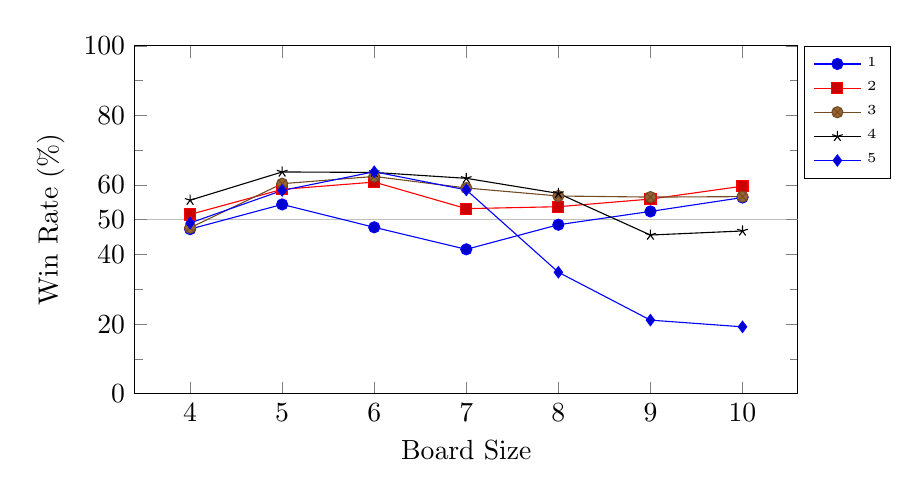
\begin{tikzpicture}
\begin{axis}[
	xlabel=Board Size,
	ylabel=Win Rate (\%),
	xtick={4,5,6,7,8,9,10},
	ymin=0, ymax=100,
	minor y tick num=1,
	extra y ticks={50},
	extra y tick style={grid=major},
]
\addplot coordinates { (4,47.31) (5,54.41) (6,47.83) (7,41.50) (8,48.57) (9,52.40) (10,56.39) }; \addlegendentry{1}
\addplot coordinates { (4,51.53) (5,58.74) (6,60.83) (7,53.20) (8,53.75) (9,55.95) (10,59.65) }; \addlegendentry{2}
\addplot coordinates { (4,47.70) (5,60.37) (6,62.45) (7,59.13) (8,56.83) (9,56.52) (10,56.65) }; \addlegendentry{3}
\addplot coordinates { (4,55.62) (5,63.74) (6,63.61) (7,61.91) (8,57.58) (9,45.61) (10,46.78) }; \addlegendentry{4}
\addplot coordinates { (4,49.08) (5,58.42) (6,63.80) (7,58.58) (8,34.92) (9,21.15) (10,19.23) }; \addlegendentry{5}
\end{axis}
\end{tikzpicture}
	\caption{Ring Rule Permanent Stones Against Baseline RAVE Player}
	\label{fig:ringperm}
\end{figure}
\end{frame}

\begin{frame}{Ring Rule: Permanent stones}
\begin{table}
	\centering
	\begin{tabular}{l|rrr}
		Size & Fork & Bridge & Ring \\ \hline
		   4 & 4212 &   5644 & 136 \\
		   5 & 5986 &   3773 & 236 \\
		   6 & 7051 &   2321 & 626 \\
		   7 & 7444 &   2132 & 422 \\
		   8 & 8283 &   1397 & 319 \\
		   9 & 8635 &    929 & 436 \\
		  10 & 8768 &    971 & 261 \\
	\end{tabular}
	\caption{Number of Wins of Each Type by Board Size Given 10000 Simulations When Only Counting Rings With Three or More Permanent Stones}
	\label{tab:wintypesperm}
\end{table}
\end{frame}



\begin{frame}{Combination}
\begin{itemize}
\item Tested using all the good features together, removing one at a time, all against the RAVE baseline.

\item The heuristic knowledge features that were included are:
%\vspace{-5mm}
\begin{itemize}
%	\setlength{\itemsep}{0pt}
%	\setlength{\parskip}{0pt}
%	\setlength{\parsep}{0pt}
\item Maintain Virtual Connections (value 100)
\item Connectivity (value 20)
\item Locality (value 3)
\item Local Reply (value 5)
\item Distance (value 2)
\item Group Size (value 2)
\end{itemize}

\item The rollout policy features that were included are:
%\vspace{-5mm}
\begin{itemize}
%	\setlength{\itemsep}{0pt}
%	\setlength{\parskip}{0pt}
%	\setlength{\parsep}{0pt}
\item Multiple rollouts (5 rollouts per simulation)
\item Mate-in-one (Only for the first N moves where N is the board size)
\item Ring Rule Depth (Only allow rings until 70\% of empty cells are filled)
\item Ring Rule Permanent Stones (Rings require 3 permanent stones)
\end{itemize}
\end{itemize}
\end{frame}

\begin{frame}{Combination, Rollouts}
\begin{figure}
	\centering
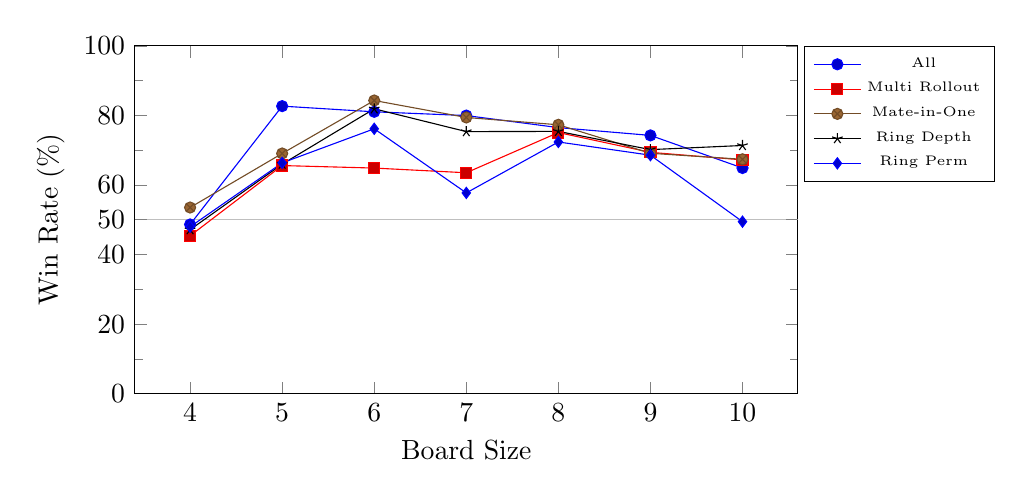
\begin{tikzpicture}
\begin{axis}[
	xlabel=Board Size,
	ylabel=Win Rate (\%),
	xtick={4,5,6,7,8,9,10},
	ymin=0, ymax=100,
	minor y tick num=1,
	extra y ticks={50},
	extra y tick style={grid=major},
]
\addplot coordinates { (4,48.65) (5,82.66) (6,81.03) (7,79.95) (8,76.49) (9,74.25) (10,64.88) }; \addlegendentry{All}
\addplot coordinates { (4,45.39) (5,65.58) (6,64.86) (7,63.51) (8,75.07) (9,69.38) (10,67.21) }; \addlegendentry{Multi Rollout}
\addplot coordinates { (4,53.52) (5,69.05) (6,84.28) (7,79.40) (8,77.30) (9,69.11) (10,67.38) }; \addlegendentry{Mate-in-One}
\addplot coordinates { (4,47.15) (5,65.99) (6,81.89) (7,75.34) (8,75.40) (9,70.16) (10,71.35) }; \addlegendentry{Ring Depth}
\addplot coordinates { (4,47.98) (5,66.35) (6,76.15) (7,57.72) (8,72.36) (9,68.56) (10,49.46) }; \addlegendentry{Ring Perm}
\end{axis}
\end{tikzpicture}
	\caption{Rollout Modifications}
	\label{fig:comborollout}
\end{figure}
\end{frame}

\begin{frame}{Combination, Knowledge}
\begin{figure}
	\centering
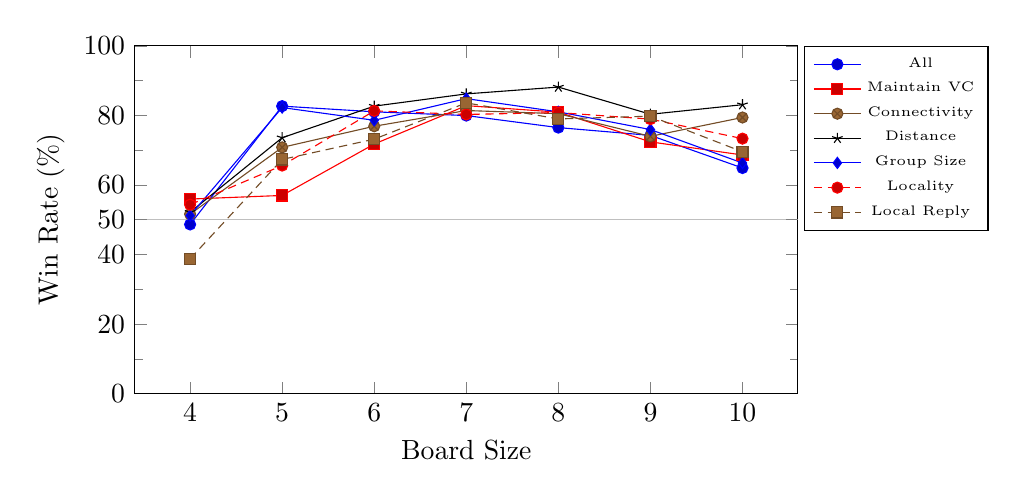
\begin{tikzpicture}
\begin{axis}[
	xlabel=Board Size,
	ylabel=Win Rate (\%),
	xtick={4,5,6,7,8,9,10},
	ymin=0, ymax=100,
	minor y tick num=1,
	extra y ticks={50},
	extra y tick style={grid=major},
]
\addplot coordinates { (4,48.65) (5,82.66) (6,81.03) (7,79.95) (8,76.49) (9,74.25) (10,64.88) }; \addlegendentry{All}
\addplot coordinates { (4,55.95) (5,56.99) (6,71.77) (7,82.80) (8,80.93) (9,72.39) (10,68.62) }; \addlegendentry{Maintain VC }
\addplot coordinates { (4,51.62) (5,70.81) (6,76.88) (7,81.40) (8,80.49) (9,73.98) (10,79.40) }; \addlegendentry{Connectivity}
\addplot coordinates { (4,52.17) (5,73.58) (6,82.66) (7,86.18) (8,88.14) (9,80.32) (10,83.07) }; \addlegendentry{Distance}
\addplot coordinates { (4,51.22) (5,82.25) (6,78.59) (7,84.82) (8,81.02) (9,75.93) (10,66.31) }; \addlegendentry{Group Size}
\addplot coordinates { (4,54.34) (5,65.58) (6,81.30) (7,80.27) (8,80.81) (9,78.92) (10,73.32) }; \addlegendentry{Locality}
\addplot coordinates { (4,38.78) (5,67.34) (6,73.17) (7,83.60) (8,78.98) (9,79.78) (10,69.54) }; \addlegendentry{Local Reply}
\end{axis}
\end{tikzpicture}
	\caption{Knowledge Modifications}
	\label{fig:comboknow}
\end{figure}
\end{frame}


%%%%%%%%%%%%%%%%%%%%%%%%%%%%%%%%%%%%%%%%%%%%%%%

\section{Solving Havannah}

\begin{frame}{Symmetry}
\begin{itemize}
\item Only 6 of the 37 cells on an empty size 4 board are unique
\item Havannah board has 12-fold symmetry
\item Store a zobrist hash for each direction
\item Take the minimum zobrist hash as the representative hash
\item Only generate one move for each symmetrical move
\item Only look for symmetry for the first 5 moves
\end{itemize}
\end{frame}

\subsection{Multi-threading}

\begin{frame}{Multi-threading}
\begin{itemize}
\item One master thread, handles GTP commands
\item Pool of player threads
\item Simple state machine: Wait\_Start, Wait\_End, Running, Garbage\_Collection, Cancelled
\item All updates done with atomic operations (CAS, atomic increment)
\item Thread local random number generator to avoid locks and memory contention
\item Virtual Loss to distribute threads around the tree
\item Pondering to make debugging easier
\end{itemize}
\end{frame}

\subsection{Memory Management}

\begin{frame}{Garbage Collection}
\begin{itemize}
\item Tree can get bigger than physical memory
\item Throw away irrelevant parts of the tree
\item Throw away any node with little experience, increasing/decreasing to garbage collect half the nodes
\item Has little impact on performance
\end{itemize}
\end{frame}

\begin{frame}{Memory Management}
\begin{itemize}
\item Can't account for overhead from malloc
\item Memory overhead increases over time due to fragmentation
\item Need strong upper bounds on memory
\item Built a compacting tree, that can move memory around as needed
\item Very fast allocation strategy
\item Every byte is accounted for
\end{itemize}
\end{frame}

\subsection{Draw Detection}


\begin{frame}{Draw Detection}
\begin{figure}
	\centering
	\begin{HavannahBoard}[board size=4,coordinate style=classical,show coordinates=false]
	\HGame{g7,a1,f5,g4,e3,d2,e2,d1,c2,d3,c3,f7,d6,b4,a4,b5,a3,e5,c4,b3, a2,c1,b1,f6,e4,d4,g6,e7,d7,b2,c5}
	\end{HavannahBoard}
	\caption{After move 30 no wins are possible}
\end{figure}
\end{frame}

\begin{frame}{Draw Detection}
\begin{itemize}
\item Proving a draw means enumerating all ways of filling these cells
\item With 7 empty cells, that's $7! = 5040$ simulations
\item Proving no bridges or forks are possible can be done with Distance to Win heuristic
\item Proving no rings are possible means checking for encirclability
	\begin{itemize}
	\item A group that touches the edge can't be encircled by the opponent
	\item Any cell next to a group that touches an edge can't be encircled
	\end{itemize}
\item If no cells can be encircled, and no bridges or forks exist, it's a draw
\end{itemize}
\end{frame}


\subsection{Solution}

\begin{frame}{Solution to Sizes 2 and 3}
\begin{figure}[tb]
\centering

	\begin{HavannahBoard}[board size=2,coordinate style=classical,show coordinates=false]
	\HStoneGroup[color=white]{a1,a2,b1,b3,c2,c3}
	\HStoneGroup[color=black]{b2}
	\end{HavannahBoard}

	\begin{HavannahBoard}[board size=3,coordinate style=classical,show coordinates=false]
	\HStoneGroup[color=white]{a1,a3,c1,c5,e3,e5}
	\HStoneGroup[color=black]{a2,b1,b2,b3,b4,c2,c3,c4,d2,d3,d4,d5,e4}
	\end{HavannahBoard}
\caption{Solution to sizes 2 and 3. The colour of a piece represents the winner if white makes the first move in that position. No openings lead to a draw.}
\end{figure}
\end{frame}


\begin{frame}{Solution to Size 4}
\begin{figure}[tb]
\centering
	\begin{HavannahBoard}[board size=4,coordinate style=classical,show coordinates=false]
	\HStoneGroup[color=white]{a1,a2,a3,a4,b1,b2,b3,b4,b5,c1,c2,c3,c4,c5,c6,d1,d2,d3,d4,d5,d6,d7,e2,e3,e4,e5,e6,e7,f3,f4,f5,f6,f7,g4,g5,g6,g7}
	\end{HavannahBoard}
\caption{Solution to size 4. The colour of a piece represents the winner if white makes the first move in that position. No openings lead to a draw.}
\end{figure}
\end{frame}

\begin{frame}{Solution to Size 4}
\begin{itemize}
\item Proven twice with MCTS
\item Takes about $4 \times 10^{11}$ simulations, or 1 week with 80 cores to solve
\item Easiest opening takes about 3-12 hours to solve, depending on how lucky it is
\item Easiest opening confirmed with Proof Number Search, took 80 hours
\item Proof trees are posted at \url{http://ualberta.ca/~tewalds/}
\item Size 4 took $6 \times 10^8$ times more time to solve than size 3, which is roughly the difference in the state space, suggesting size 5 will take $10^{12}$ more effort to solve than size 4.
\end{itemize}
\end{frame}

%\begin{frame}{Proof Tree a1}
%\begin{figure}
%\centering
%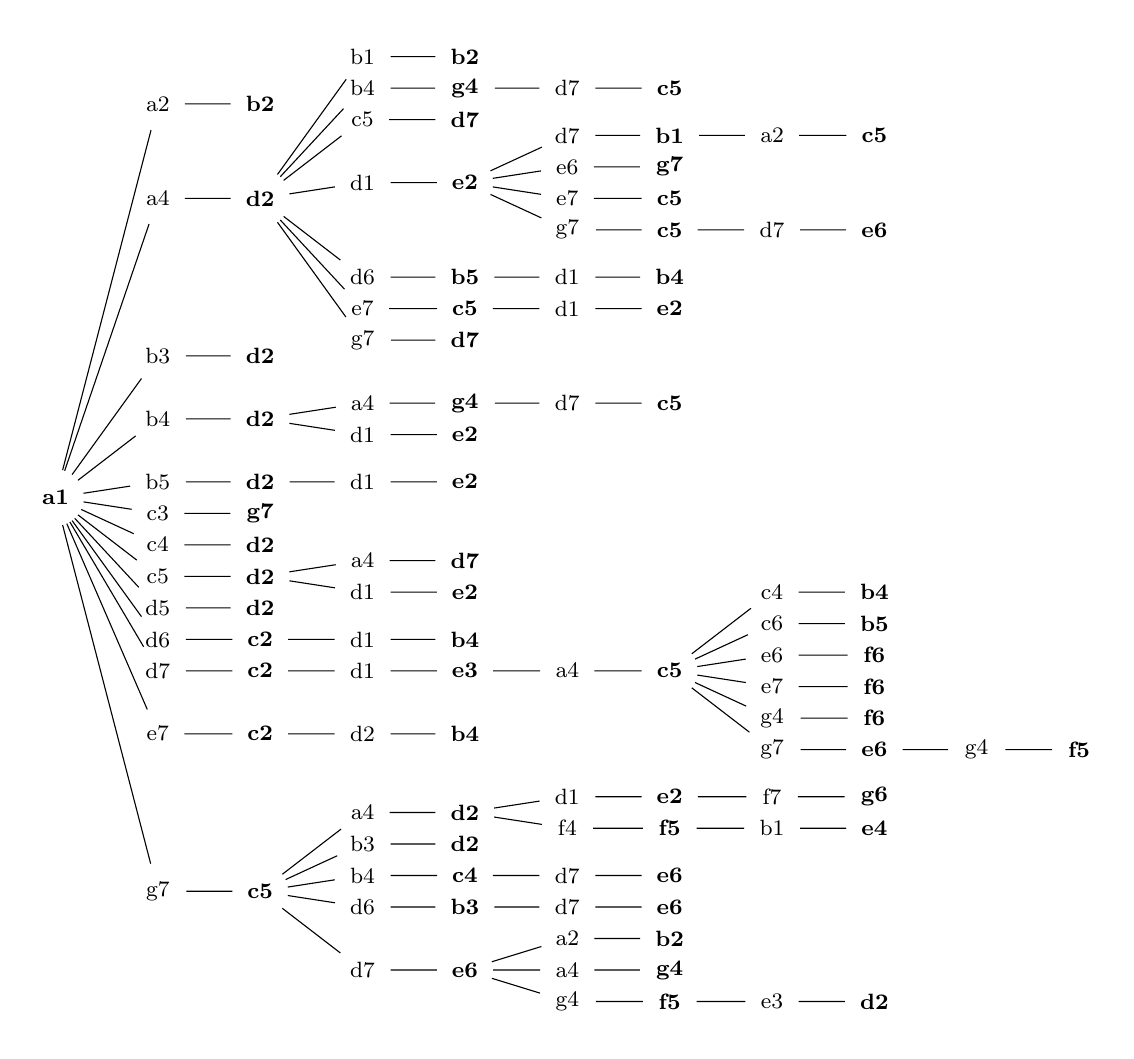
\begin{tikzpicture}[
	font=\footnotesize,
	grow'=right,
	level distance=13mm,
	level 1/.style={sibling distance=4mm},
	level 2/.style={sibling distance=4mm},
	level 3/.style={sibling distance=4mm},
	ww/.style={circle,font=\footnotesize\bfseries},
	wb/.style={circle},
	bw/.style={circle},
	bb/.style={circle,font=\footnotesize\bfseries},
	]
\node [ww] {a1}
	child { node [bw] {a2}
		child { node [ww] {b2} }
	}
	child [missing] foreach \a in {1,...,2} { }
	child { node [bw] {a4}
		child { node [ww] {d2}
			child { node [bw] {b1}
				child { node [ww] {b2} }
			}
			child { node [bw] {b4}
				child { node [ww] {g4}
					child { node [bw] {d7}
						child { node [ww] {c5} }
					}
				}
			}
			child { node [bw] {c5}
				child { node [ww] {d7} }
			}
			child [missing] foreach \a in {1,...,1} { }
			child { node [bw] {d1}
				child { node [ww] {e2}
					child { node [bw] {d7}
						child { node [ww] {b1}
							child { node [bw] {a2}
								child { node [ww] {c5} }
							}
						}
					}
					child { node [bw] {e6}
						child { node [ww] {g7} }
					}
					child { node [bw] {e7}
						child { node [ww] {c5} }
					}
					child { node [bw] {g7}
						child { node [ww] {c5}
							child { node [bw] {d7}
								child { node [ww] {e6} }
							}
						}
					}
				}
			}
			child [missing] foreach \a in {1,...,2} { }
			child { node [bw] {d6}
				child { node [ww] {b5}
					child { node [bw] {d1}
						child { node [ww] {b4} }
					}
				}
			}
			child { node [bw] {e7}
				child { node [ww] {c5}
					child { node [bw] {d1}
						child { node [ww] {e2} }
					}
				}
			}
			child { node [bw] {g7}
				child { node [ww] {d7} }
			}
		}
	}
	child [missing] foreach \a in {1,...,4} { }
	child { node [bw] {b3}
		child { node [ww] {d2} }
	}
	child [missing] foreach \a in {1,...,1} { }
	child { node [bw] {b4}
		child { node [ww] {d2}
			child { node [bw] {a4}
				child { node [ww] {g4}
					child { node [bw] {d7}
						child { node [ww] {c5} }
					}
				}
			}
			child { node [bw] {d1}
				child { node [ww] {e2} }
			}
		}
	}
	child [missing] foreach \a in {1,...,1} { }
	child { node [bw] {b5}
		child { node [ww] {d2}
			child { node [bw] {d1}
				child { node [ww] {e2} }
			}
		}
	}
	child { node [bw] {c3}
		child { node [ww] {g7} }
	}
	child { node [bw] {c4}
		child { node [ww] {d2} }
	}
	child { node [bw] {c5}
		child { node [ww] {d2}
			child { node [bw] {a4}
				child { node [ww] {d7} }
			}
			child { node [bw] {d1}
				child { node [ww] {e2} }
			}
		}
	}
	child { node [bw] {d5}
		child { node [ww] {d2} }
	}
	child { node [bw] {d6}
		child { node [ww] {c2}
			child { node [bw] {d1}
				child { node [ww] {b4} }
			}
		}
	}
	child { node [bw] {d7}
		child { node [ww] {c2}
			child { node [bw] {d1}
				child { node [ww] {e3}
					child { node [bw] {a4}
						child { node [ww] {c5}
							child { node [bw] {c4}
								child { node [ww] {b4} }
							}
							child { node [bw] {c6}
								child { node [ww] {b5} }
							}
							child { node [bw] {e6}
								child { node [ww] {f6} }
							}
							child { node [bw] {e7}
								child { node [ww] {f6} }
							}
							child { node [bw] {g4}
								child { node [ww] {f6} }
							}
							child { node [bw] {g7}
								child { node [ww] {e6}
									child { node [bw] {g4}
										child { node [ww] {f5} }
									}
								}
							}
						}
					}
				}
			}
		}
	}
	child [missing] foreach \a in {1,...,1} { }
	child { node [bw] {e7}
		child { node [ww] {c2}
			child { node [bw] {d2}
				child { node [ww] {b4} }
			}
		}
	}
	child [missing] foreach \a in {1,...,4} { }
	child { node [bw] {g7}
		child { node [ww] {c5}
			child { node [bw] {a4}
				child { node [ww] {d2}
					child { node [bw] {d1}
						child { node [ww] {e2}
							child { node [bw] {f7}
								child { node [ww] {g6} }
							}
						}
					}
					child { node [bw] {f4}
						child { node [ww] {f5}
							child { node [bw] {b1}
								child { node [ww] {e4} }
							}
						}
					}
				}
			}
			child { node [bw] {b3}
				child { node [ww] {d2} }
			}
			child { node [bw] {b4}
				child { node [ww] {c4}
					child { node [bw] {d7}
						child { node [ww] {e6} }
					}
				}
			}
			child { node [bw] {d6}
				child { node [ww] {b3}
					child { node [bw] {d7}
						child { node [ww] {e6} }
					}
				}
			}
			child [missing] foreach \a in {1,...,1} { }
			child { node [bw] {d7}
				child { node [ww] {e6}
					child { node [bw] {a2}
						child { node [ww] {b2} }
					}
					child { node [bw] {a4}
						child { node [ww] {g4} }
					}
					child { node [bw] {g4}
						child { node [ww] {f5}
							child { node [bw] {e3}
								child { node [ww] {d2} }
							}
						}
					}
				}
			}
		}
	}
;
\end{tikzpicture}


%\caption[Proof Tree for the a1 Opening on Size 4]{Proof Tree for the a1 opening on size 4 showing nodes that took more than $10^8$ simulations to solve}
%\end{figure}
%\end{frame}

%%%%%%%%%%%%%%%%%%%%%%%%%%%%%%%%%%%%%%%%%%%%%%%

\section{Conclusion}

\subsection{Conclusion}

\begin{frame}{Conclusion}
\begin{itemize}
\item
\item
\item
\item
\item
\item
\end{itemize}
\end{frame}

\subsection{Future Work}

\begin{frame}{Future Work}
\begin{itemize}
\item
\item
\item
\item
\item
\item
\end{itemize}
\end{frame}


\begin{frame}{Questions?}
\end{frame}


\end{document}

